\documentclass[germanthesis]{thesis-style}
% options:
% [germanthesis] - Thesis is written in German
% [plainunnumbered] - Don't print numbers on plain pages
% [earlydraft] - Settings for quick draft printouts
% [watermark] - Print current time/date at bottom of each page
% [phdthesis] - switch to PhD thesis style
% [twoside] - double sided
% [cutmargins] - text body fills complete page

% Extension to BibLaTex (useful for cites in footnotes)
%\usepackage[backend=bibtex, style=numeric-comp]{biblatex}
\bibliography{references}

\author{Martin~Nocker}
\title{R-Paket für Kanalkodierung mit Faltungskodes}
%\title{R~package for channel~coding with convolutional~codes}
\birthday{1. Mai 1993}
\birthplace{Innsbruck}
%\thesisstart{20. Oktober 2015}
\thesistype{Bachelor's thesis}
\thesistypegerman{Bachelorarbeit}
\thesiscite{Bachelor's thesis}
\advisors{Univ.-Prof.~Dr.~Rainer~Böhme, Dr.~Pascal~Schöttle}

% additional packages
\usepackage{color, colortbl} % colors (interface table)
\usepackage{longtable}
\usepackage{amsmath}
\usepackage{graphicx}
\usepackage{caption}
\usepackage{subcaption}
\usepackage{tikz}
\usetikzlibrary{backgrounds, calc, positioning}

% Caption von longtables ändern (Tabelle -> Funktion)
\captionsetup[longtable]{name=Funktion}

% Listings standardmaessig in R
\lstset{language=R}

% Theorems
\usepackage{amsthm}
\newtheorem*{thm_massey_sain}{Theorem von Massey-Sain}

% Definiert Makro für Grafik Skalierung
\makeatletter
\def\ScaleIfNeeded{%
\ifdim\Gin@nat@width>\linewidth
\linewidth
\else
\Gin@nat@width
\fi
}
\makeatother

\newcommand{\plotwidth}{0.6\textwidth}
\begin{document}

% Titelseiten und Eidesstattliche Erklärung
\maketitle

% Zusammenfassung
\begin{abstract}

\end{abstract}

\tableofcontents
\clearpage
\pagenumbering{arabic}

\chapter{Einleitung}
\label{kapitel:einleitung}
% einleitung.tex
Kanalkodierung stellt, aufgrund der stetigen Ausbreitung digitaler Kommunikationssysteme, ein wichtiges Teilgebiet der Kodierungstheorie dar. Informationen, die über einen Kanal zwischen Quelle und Empfänger übertragen werden, können aufgrund von Rauschen verändert werden. Die Kanalkodierung stellt Methoden zur Verfügung, um Fehler, die während der Übertragung über einen verrauschten Kanal auftreten, zu korrigieren. Verwendung findet die Kanalkodierung in der Mobil- und Satellitenkommunikation, da beispielsweise das erneute Senden von Satellitendaten, bei Auftreten von Rauschen, aufgrund der Laufzeiten unpraktisch wäre. Weiters wird die Kanalkodierung zur Speicherung von Daten, etwa auf Compact-Disks, verwendet. Rauschen kann durch thermische Störungen bzw. Kratzer oder Fingerabdrücke auf Compact-Disks hervorgerufen werden.

Eine Art der Kanalkodierung stellen Faltungskodes dar, auf welche sich diese Arbeit konzentriert. Die wichtigste Anwendung von Faltungskodes ist die Konstruktion von Turbo-Kodes, welche eine Erweiterung der Faltungskodes darstellen. Weiters existiert mit Blockkodes ein weiteres wichtiges Verfahren der Kanalkodierung.
\\
\\
Ziel dieser Arbeit ist die Implementierung von Faltungskodes mithilfe der Programmiersprache R. Das entwickelte R-Paket dient zukünftigen Studierenden zu Lehrzwecken und soll sie beim Studieren von Faltungskodes unterstützen. Studierenden soll dadurch, neben den theoretischen Grundlagen im Zuge einer Vorlesung, eine praktische Möglichkeit zur Anwendung von Faltungskodes geboten werden. Mithilfe dynamisch generierter Visualisierungen, sollen die Prinzipien von Faltungskodes vermittelt werden.

Die Arbeiten \enquote{R-Paket für Kanalkodierung mit Blockkodes}~\cite{wimmer} von Benedikt Wimmer und \enquote{R-Paket für Kanalkodierung mit Turbo-Kodes}~\cite{witsch} von Daniel Witsch stellen Implementierungen der Blockkodes bzw. Turbo-Kodes zur Verfügung, die ebenfalls im Paket enthalten sind. Dadurch ergibt sich ein sowohl umfangreiches als auch kompaktes Paket der Kanalkodierung.

\chapter{Grundlagen und ähnliche Arbeiten}
\label{kapitel:grundlagen}
% grundlagen.tex
In diesem Kapitel werden die theoretischen Grundlagen eingeführt. In Kapitel~\ref{kapitel:grundlagen_kanalkodierung} werden Prinzipien und Eigenschaften der Kanalkodierung beschrieben. Kapitel~\ref{kapitel:grundlagen_faltungskodierung} geht auf Faltungskodes ein, eine Art der Kanalkodierung auf die sich diese Arbeit konzentriert.
\section{Kanalkodierung}
\label{kapitel:grundlagen_kanalkodierung}
\begin{figure}[t]
\centering
\resizebox{\textwidth}{!}{%
	% kommunikationskanal.tex
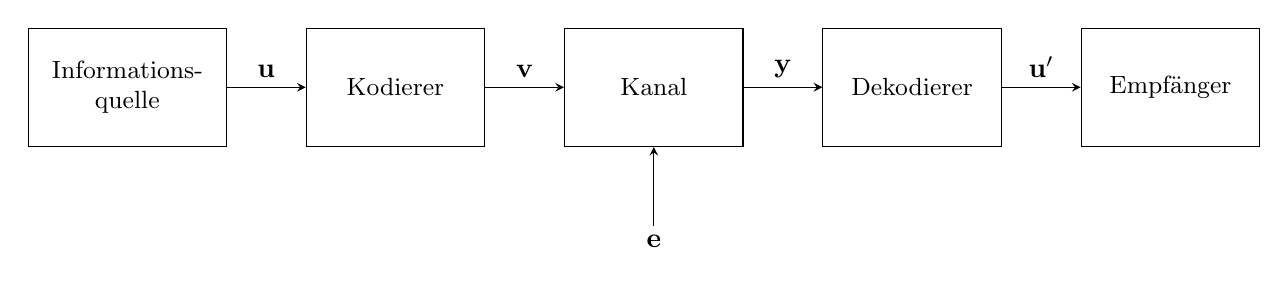
\begin{tikzpicture}[>=stealth]
\def\myinnersep{3mm}
\tikzstyle{block} = [draw, rectangle, node distance=10mm, inner sep=\myinnersep, align=center, font=\small, minimum height=15mm, minimum width=width("Dekodierer")+2*\myinnersep]
\node[block] (quelle) {Informations- \\ quelle};
\node[block] (kodierer) [right=of quelle] {Kodierer};
\node[block] (kanal) [right=of kodierer] {Kanal};
\node[block] (dekodierer) [right=of kanal] {Dekodierer};
\node[block] (senke) [right=of dekodierer] {Empfänger};
\draw[->] (quelle) -- node [above] {$\mathbf{u}$} (kodierer);
\draw[->] (kodierer) -- node [above] {$\mathbf{v}$} (kanal);
\draw[->] (kanal) -- node [above] {$\mathbf{y}$} (dekodierer);
\draw[->] (dekodierer) -- node [above] {$\mathbf{u'}$} (senke);
\draw[<-] (kanal.south) -- ++(0,-10mm) node [below] {$\mathbf{e}$};
\end{tikzpicture}
}
\caption{Kommunikationskanal}
\label{abb:kommunikationskanal}
\end{figure}
Kanalkodierung kann als Zuordnung bzw. Abbildung von Quellzeichen (Zeichen die eine Informationsquelle emittiert) zu Kanalzeichen (Zeichen die über den Kommunikationskanal übertragen werden) angesehen werden. Der Kanal enthält ein Rauschen, d.h. Informationen die von der Quelle emittiert werden, können verändert beim Empfänger ankommen. Daher wird der Kanal auch als \emph{verrauschter} Kanal bezeichnet. Würde eine Information unkodiert über den verrauschten Kanal übertragen werden, kann die verfälschte Nachricht nicht wiederhergestellt werden. Daher fügt der Kanalkodierer den Quellzeichen Redundanz hinzu, sodass empfängerseitig verfälschte Zeichen erkannt und korrigiert werden können. Abbildung~\ref{abb:kommunikationskanal} zeigt einen Kommunikationskanal inklusive Kanalkodierung. 

Eine Nachricht $\mathbf{u}=\left( u_{1},u_{2},\dots ,u_{k}\right)$ wird in ein Kodewort $\mathbf{v}=\left( v_{1},v_{2},\dots ,v_{n}\right)$, das Redundanz enthält, kodiert. Vor der Übertragung über den Kanal werden die Bits auf die Signalpegel +1 bzw. -1 folgendermaßen abgebildet:
\begin{equation}
\text{Signal(Bit)} =
\begin{cases}
  +1  & \quad \text{wenn Bit} = 0\\
  -1  & \quad \text{wenn Bit} = 1\\
\end{cases}
\label{eq:bit_zu_signal_abbildung}
\end{equation}
Bei der Übertragung wird das Signal durch Rauschen, welches als Fehlervektor $\mathbf{e}=\left( e_{1},e_{2},\dots ,e_{n}\right)$ dargestellt wird, verfälscht. Der Empfangsvektor$\mathbf{y}$ ergibt sich aus der Überlagerung von $\mathbf{v}$ und $\mathbf{e}$. Der Empfangsvektor wird vor der Dekodierung von den Signalpegel zurück auf die Bit-Werte 0 bzw. 1 abgebildet.
\begin{equation}
\text{Kode(Signal)} =
\begin{cases}
  0  & \quad \text{wenn Signal } \geq 0\\
  1  & \quad \text{sonst}\\
\end{cases}
\label{eq:signal_zu_bit_abbildung}
\end{equation}
Das daraus resultierende Kodewort wird vom Dekodierer zur Schätzung $\mathbf{u'}$ der originalen Nachricht dekodiert. Ziel der Kanalkodierung ist es die Wahrscheinlichkeit, dass $\mathbf{u'}=\mathbf{u}$ ist, zu maximieren.

\subsection{Koderate}
\label{kapitel:grundlagen_koderate}
Die Koderate $R$ eines Kodes beschreibt das Verhältnis der Länge zwischen Quellwort $\mathbf{u}=\left( u_{1},u_{2},\dots ,u_{k}\right)$ und Kodewort $\mathbf{v}=\left( v_{1},v_{2},\dots ,v_{n}\right)$.
\begin{equation}
R=\frac{k}{n}<1
\end{equation}
In anderen Worten beschreibt die Koderate das Verhältnis zwischen Information und Redundanz im übertragenen Kodewort. Bei hoher Redundanz ergibt sich eine niedrige Koderate. Die Übertragung ein und derselben Information bei gleicher Übertragungsgeschwindigkeit dauert bei Kodes mit niedriger Koderate länger, als bei Kodes mit höherer Koderate.

\subsection{Hamming-Distanz}
\label{kapitel:grundlagen_hamming_distanz}
Die Hamming-Distanz $d$ (auch $d_{H}$) zweier Kodewörter $\mathbf{a}=\left( a_{1},a_{2},\dots ,a_{n}\right)$ und $\mathbf{b}=\left( b_{1},b_{2},\dots ,b_{n}\right)$ entspricht der Anzahl an Stellen in denen sich die beiden Kodewörter unterscheiden:
\begin{equation}
d(a,b)=\vert\left\lbrace i \in \left\lbrace 1,2,\dots ,n \right\rbrace\vert a_{i}\neq b_{i}\right\rbrace\vert.
\end{equation}
Für binäre Kodewörter ergibt sich die Hamming-Distanz aus der binären Addition der Kodewörter:
\begin{equation}
d(a,b)=\sum_{i=1}^{n} \left( a_{i} \oplus b_{i}\right).
\end{equation}

\subsection{Hamming-Gewicht}
\label{kapitel:grundlagen_hamming_gewicht}
Das Hamming-Gewicht $w$ eines binären Kodeworts $\mathbf{a}=\left( a_{1},a_{2},\dots ,a_{n}\right)$ entspricht der Anzahl an 1 im Wort:
\begin{equation}
w(a)=\sum_{i=1}^{n} a_{i}.
\end{equation}

\section{Faltungskodierung}
\label{kapitel:grundlagen_faltungskodierung}
Faltungskodes sind blockfreie Kodes, d.h. Quellzeichen werden nicht in Blöcke fester Länge unterteilt, sondern es wird ein Informationsstrom kodiert, sodass ein einziges Kodewort resultiert. Ein weiterer Unterschied zu Blockkodes besteht darin, dass Kodebits nicht nur vom aktuellen Eingangsbit abhängen, sondern auch von vorherigen Eingangsbits. Die Redundanz wird bei Faltungskodes kontinuierlich in das Kodewort eingefügt. Im Allgemeinen können Faltungskodierer beliebig viele Eingänge haben. Trotz besserer Koderate bei Kodierern mit mehreren Eingängen sind nur Kodierer mit einem Eingang von praktischer Relevanz. Im Folgenden werden nur noch Faltungskodierer mit einem Eingang betrachtet.

\subsection{Kodiererdarstellung und Kodierung}
\label{kapitel:grundlagen_darstellung}
Faltungskodierer lassen sich einfach durch ein Schieberegister und mehrere logische XOR-Gatter darstellen. Bei einem Faltungskodierer mit $N$ Ausgängen und einem Schieberegister der Länge $M$ wird ein Eingangsbit $u \in \left\lbrace 0,1 \right\rbrace$ in eine Kodesequenz $\mathbf{v}$ der Länge $N$ $\left( \mathbf{v} \in {\left\lbrace 0,1\right\rbrace }^{N}\right)$ kodiert. Es ergibt sich somit eine Koderate von $R=\frac{1}{N}$. Ein Ausgang wird durch ein sogenanntes \emph{Generatorpolynom} definiert. Dieses stellt eine Linearkombination der $M$ Elemente des Schieberegisters und dem Eingangssignal dar und werden durch die XOR-Gatter abgebildet. Alle Generatorpolynome werden in einer \emph{Generatormatrix}
\begin{equation}
G=\left( g_{1}, g_{2},\dots , g_{N} \right) 
\end{equation}
angegeben, wobei das Generatorpolynom $g_{i}$ Ausgang $i$ definiert. Zur Definition eines Faltungskodierers im späteren Programm müssen die oktalen Generatorpolynome angegeben werden.
\\
Ein weiterer wichtiger Parameter von Faltungskodes ist die \emph{Einflusslänge} (constraint length) die angibt wie oft sich ein Eingangsbit auf die Kodierung auswirkt und wird durch die Länge des Schieberegisters bestimmt. Ein Eingangsbit beeinflusst $M+1$ mal die Kodierung.
\\
\\
Die Verhaltensweise eines Faltungskodierers kann weiters durch seinen \emph{Zustandsgraphen} beschrieben werden. Ein Zustand entspricht einer bestimmten Bitbelegung des Schieberegisters. Für einen Faltungskodierer mit einem Schieberegister der Länge $M$ ergeben sich $2^{M}$ Zustände. Faltungskodierer starten, falls nicht explizit angegeben, im Nullzustand, d.h. die Elemente des Schieberegisters sind mit 0 initialisiert.
\begin{figure}[t]
	\centering
	\begin{subfigure}{0.65\textwidth}
		\centering
		\resizebox{0.99\textwidth}{!}{%
			% standardkodierer.tex
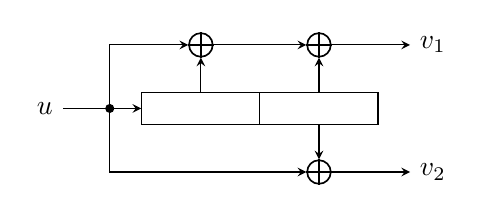
\begin{tikzpicture}[>=stealth]
\tikzstyle{rect} = [draw, rectangle, minimum width=30mm, inner sep=0mm, minimum height=4mm]
\tikzstyle{xor} = [draw, circle, semithick, minimum size=3mm, inner sep=0mm]

\node[rect] (rect) {};
\draw[-] (rect.north) -- (rect.south);
\draw[<-] (rect.west) -- ++(-10mm,0) node [left] {$u$};

\node[xor] (xor1) at ($(rect.north)+(-7.5mm,6mm)$) {};
\draw[semithick] (xor1.north) -- (xor1.south);
\draw[semithick] (xor1.west) -- (xor1.east);
\draw[->] ($(rect.north)+(-7.5mm,0)$) -- (xor1.south);

\node[xor] (xor2) at ($(rect.north)+(7.5mm,6mm)$) {};
\draw[semithick] (xor2.north) -- (xor2.south);
\draw[semithick] (xor2.west) -- (xor2.east);
\draw[->] ($(rect.north)+(7.5mm,0)$) -- (xor2.south);

\node[xor] (xor3) at ($(rect.south)+(7.5mm,-6mm)$) {};
\draw[semithick] (xor3.north) -- (xor3.south);
\draw[semithick] (xor3.west) -- (xor3.east);
\draw[->] ($(rect.south)+(7.5mm,0)$) -- (xor3.north);

\draw[->] ($(rect.west)+(-4mm,0)$) |- (xor1.west);
\draw[->] (xor1.east) -- (xor2.west);
\draw[->] (xor2.east) -- ($(rect.north east)+(4mm,6mm)$) node [right] {$v_{1}$};

\draw[->] ($(rect.west)+(-4mm,0)$) |- (xor3.west);
\draw[->] (xor3.east) -- ($(rect.south east)+(4mm,-6mm)$) node [right] {$v_{2}$};

\draw[black, fill=black] ($(rect.west)+(-4mm,0)$) circle [radius=.5mm];
\end{tikzpicture}
		}
		\caption{Schaltbild}
	\end{subfigure}
	~ % spacing between subfigures
	\begin{subfigure}{0.3\textwidth}
		\centering
		\resizebox{0.99\textwidth}{!}{%
			% zustandsdiagramm.tex
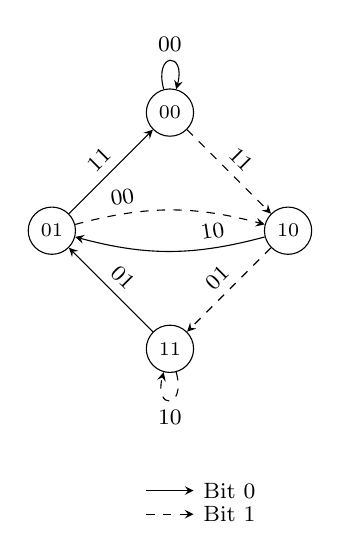
\begin{tikzpicture}[>=stealth, font=\footnotesize, scale=.6]
\tikzstyle{state} = [draw, circle, inner sep=1mm, minimum size=6mm, font=\scriptsize]
\node[state] (state0) at ( 0.0, 2.5) {$00$};
\node[state] (state2) at ( 2.5, 0.0) {$10$};
\node[state] (state3) at ( 0.0,-2.5) {$11$};
\node[state] (state1) at (-2.5, 0.0) {$01$};
\draw[->] (state0) to [looseness=8,out=105,in=75] node [sloped, above] {$00$} (state0);
\draw[->, dashed] (state0) to  node [sloped, above] {$11$} (state2);
\draw[->] (state1) to  node [sloped, above] {$11$} (state0);
\draw[->, dashed] (state1) to [bend left=15] node [sloped, above,near start] {$00$} (state2);
\draw[->] (state2) to [bend left=15] node [sloped, above,near start] {$10$} (state1);
\draw[->, dashed] (state2) to  node [sloped, above] {$01$} (state3);
\draw[->] (state3) to  node [sloped, above] {$01$} (state1);
\draw[->, dashed] (state3) to [looseness=8,out=285,in=255] node [sloped, below] {$10$} (state3);
\draw [->] ($(state3)+(-.5,-3)$) node (bit0) {} -- ++(1,0) node [right] {Bit 0};
\draw [->, dashed] ($(bit0)+(0,-.5)$) -- ++(1,0) node [right] {Bit 1};
\end{tikzpicture}
		}
		\caption{Zustandsdiagramm}
	\end{subfigure}
	\caption{Beispiel für Faltungskodierer}
	\label{abb:standardkodierer}
\end{figure}
\begin{beispiel} Ein Faltungskodierer ist gegeben durch das Schaltbild bzw. Zustandsdiagramm in Abbildung~\ref{abb:standardkodierer}. Der Faltungskodierer besitzt die Generatormatrix 
\begin{equation*}
G=\left(7_{8},5_{8}\right) = \begin{pmatrix}
111 \\
101 \\
\end{pmatrix} = \left(1+D+D^{2}, 1+D^{2} \right)
\end{equation*}
\label{bsp:B1}
\end{beispiel}
Beispiel~\ref{bsp:B1} zeigt die verschiedenen Notationen für die Generatormatrix. Die am häufigsten verwendete Schreibweise ist die Darstellung der Generatorpolynome in oktaler Form. Dabei werden die Polynome in binärer Schreibweise konzise zu oktalen Zahlen zusammengefasst. Bei der binären Schreibweise entspricht die Bitposition des Polynoms dem Element im Schaltbild, d.h. das MSB\footnote{Most Significant Bit} des Polynoms steht für das Eingangssignal, das LSB\footnote{Least Significant Bit} des Polynoms steht für den Inhalt des letzten (am weitesten rechts liegende) Element des Schieberegisters. In die Linearkombination zur Definition des Ausgangssignals werden jene Elemente miteinbezogen, an deren Stelle im binären Polynom eine 1 steht. \cite{huffman2010fundamentals} führt als Notation die binären Polynome über der Variable $D$ (\enquote{delay}) ein. Das Eingangssignal und die Schieberegisterelemente entsprechen einer Potenz von $D$, wobei das Eingangssignal $D^{0}$ und das letzte Schieberegisterelement $D^{M}$ entspricht. Das Generatorpolynom entspricht der Summe aller Potenzen deren Elemente Teil der Linearkombination sind.
\\
Weiters wird das Zustandsdiagramm abgebildet. Die Knoten stellen die Zustände des Kodierer, d.h. die Belegungen des Schieberegisters, dar. Die gerichteten Kanten entsprechen einem Übergang bei einem Eingangsbit, wobei eine durchgezogene Kante einer 0 als Eingangsbit entspricht, eine gestrichelte Kante einer 1. Die Kantenbewertungen entsprechen den Ausgangsbits.

\begin{beispiel} Gegeben sei der Faltungskodierer aus Beispiel~\ref{bsp:B1}. Eine Nachricht $\mathbf{u}=\left( 110100\right)$ wird in den Kode $\mathbf{v}=\left( 11~01~01~00~10~11\right)$ kodiert.
\label{bsp:B2}
\end{beispiel}

\subsection{Dekodierung}
\label{kapitel:grundlagen_dekodierung}
\begin{figure}[t]
	\centering
	%\resizebox{\textwidth}{!}{%
		% trellis_kodierung.tex
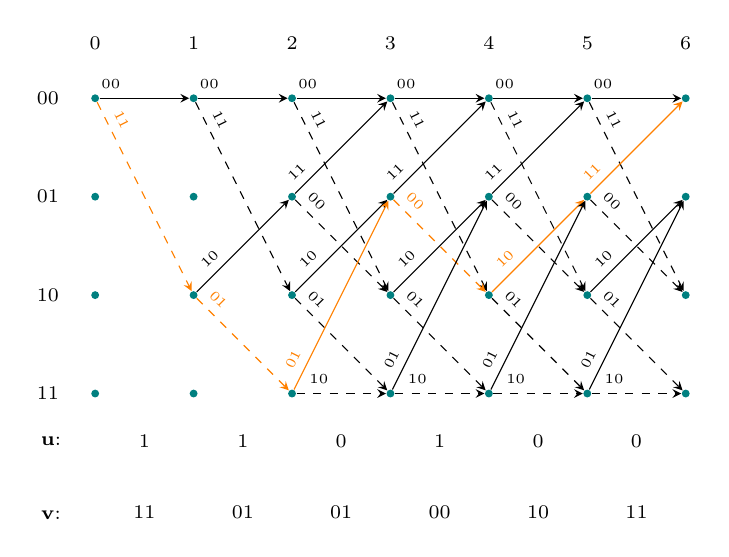
\begin{tikzpicture}[>=stealth, font=\scriptsize]
\tikzstyle{freestate} = [circle, teal, fill=teal, minimum size=1mm, inner sep=0mm]

\foreach \y in {0,...,3}
	\foreach \x in {0,...,6}
		\node[freestate] (node\y\x) at (1.25*\x,-1.25*\y) {};

\foreach \x in {0,...,6}
	\node (timelabel\x) [above of=node0\x, yshift=-3mm] {\x};
		
\node (statelabel0) [left of=node00, xshift=4mm] {00}; 
\node (statelabel1) [left of=node10, xshift=4mm] {01}; 
\node (statelabel2) [left of=node20, xshift=4mm] {10}; 
\node (statelabel3) [left of=node30, xshift=4mm] {11};

%t=0
\draw[->] (node00) -- (node01) node [sloped, above, very near start, font=\tiny] {00};
\draw[->, dashed, orange] (node00) -- (node21) node [sloped, above, very near start, font=\tiny] {11};

%t=1
\draw[->] (node01) -- (node02) node [sloped, above, very near start, font=\tiny] {00};
\draw[->, dashed] (node01) -- (node22) node [sloped, above, very near start, font=\tiny] {11};
\draw[->] (node21) -- (node12) node [sloped, above, near start, font=\tiny] {10};
\draw[->, dashed, orange] (node21) -- (node32) node [sloped, above, very near start, font=\tiny] {01};

%t=2
\draw[->] (node02) -- (node03) node [sloped, above, very near start, font=\tiny] {00};
\draw[->, dashed] (node02) -- (node23) node [sloped, above, very near start, font=\tiny] {11};
\draw[->] (node12) -- (node03) node [sloped, above, very near start, font=\tiny] {11};
\draw[->, dashed] (node12) -- (node23) node [sloped, above, very near start, font=\tiny] {00};
\draw[->] (node22) -- (node13) node [sloped, above, near start, font=\tiny] {10};
\draw[->, dashed] (node22) -- (node33) node [sloped, above, very near start, font=\tiny] {01};
\draw[->, orange] (node32) -- (node13) node [sloped, above, very near start, font=\tiny] {01};
\draw[->, dashed] (node32) -- (node33) node [sloped, above, near start, font=\tiny] {10};

%t=3
\draw[->] (node03) -- (node04) node [sloped, above, very near start, font=\tiny] {00};
\draw[->, dashed] (node03) -- (node24) node [sloped, above, very near start, font=\tiny] {11};
\draw[->] (node13) -- (node04) node [sloped, above, very near start, font=\tiny] {11};
\draw[->, dashed, orange] (node13) -- (node24) node [sloped, above, very near start, font=\tiny] {00};
\draw[->] (node23) -- (node14) node [sloped, above, near start, font=\tiny] {10};
\draw[->, dashed] (node23) -- (node34) node [sloped, above, very near start, font=\tiny] {01};
\draw[->] (node33) -- (node14) node [sloped, above, very near start, font=\tiny] {01};
\draw[->, dashed] (node33) -- (node34) node [sloped, above, near start, font=\tiny] {10};

%t=4
\draw[->] (node04) -- (node05) node [sloped, above, very near start, font=\tiny] {00};
\draw[->, dashed] (node04) -- (node25) node [sloped, above, very near start, font=\tiny] {11};
\draw[->] (node14) -- (node05) node [sloped, above, very near start, font=\tiny] {11};
\draw[->, dashed] (node14) -- (node25) node [sloped, above, very near start, font=\tiny] {00};
\draw[->,orange] (node24) -- (node15) node [sloped, above, near start, font=\tiny] {10};
\draw[->, dashed] (node24) -- (node35) node [sloped, above, very near start, font=\tiny] {01};
\draw[->] (node34) -- (node15) node [sloped, above, very near start, font=\tiny] {01};
\draw[->, dashed] (node34) -- (node35) node [sloped, above, near start, font=\tiny] {10};

%t=5
\draw[->] (node05) -- (node06) node [sloped, above, very near start, font=\tiny] {00};
\draw[->, dashed] (node05) -- (node26) node [sloped, above, very near start, font=\tiny] {11};
\draw[->,orange] (node15) -- (node06) node [sloped, above, very near start, font=\tiny] {11};
\draw[->, dashed] (node15) -- (node26) node [sloped, above, very near start, font=\tiny] {00};
\draw[->] (node25) -- (node16) node [sloped, above, near start, font=\tiny] {10};
\draw[->, dashed] (node25) -- (node36) node [sloped, above, very near start, font=\tiny] {01};
\draw[->] (node35) -- (node16) node [sloped, above, very near start, font=\tiny] {01};
\draw[->, dashed] (node35) -- (node36) node [sloped, above, near start, font=\tiny] {10};

% input & output
\node (in0) at($(node30)!0.5!(node31)+(0,-.6)$) {1};
\node (in1) at($(node31)!0.5!(node32)+(0,-.6)$) {1};
\node (in2) at($(node32)!0.5!(node33)+(0,-.6)$) {0};
\node (in3) at($(node33)!0.5!(node34)+(0,-.6)$) {1};
\node (in4) at($(node34)!0.5!(node35)+(0,-.6)$) {0};
\node (in5) at($(node35)!0.5!(node36)+(0,-.6)$) {0};
\node (inlabel) at($(node30)+(-.56,-.6)$) {$\mathbf{u}$:};

\node (out0) [below=of in0, yshift=5mm] {11};
\node (out1) [below=of in1, yshift=5mm] {01};
\node (out2) [below=of in2, yshift=5mm] {01};
\node (out3) [below=of in3, yshift=5mm] {00};
\node (out4) [below=of in4, yshift=5mm] {10};
\node (out5) [below=of in5, yshift=5mm] {11};
\node (outlabel) at($(node30)+(-.56,-1.55)$) {$\mathbf{v}$:};

\end{tikzpicture}
	%}
\caption{Trellis für die Kodierung aus Beispiel~\ref{bsp:B2}.}
\label{abb:trellis_kodierung}
\end{figure}
Zur Dekodierung von Faltungskodes wird der \emph{Viterbi-Algorithmus} angewendet. Der Algorithmus verwendet zur Dekodierung einer Kodesequenz das \emph{Trellis-Diagramm} (kurz: Trellis). Abbildung~\ref{abb:trellis_kodierung} zeigt das Trellis zur Kodierung der Nachricht aus Beispiel~\ref{bsp:B2}.
\\
Das Trellis ist eine Erweiterung des Zustandsdiagramms um eine Zeitachse (x-Achse). Die Zustände sind auf der y-Achse aufgetragen. Das Diagramm startet wie die Kodierung im Nullzustand. Ein durchgezogener Pfeil entspricht einer 1 als Eingangsbit, ein gestrichelter Pfeil einer 0 als Eingangsbit. Die Pfeile sind wiederum mit den entsprechenden Ausgangsbits, die das Kodewort ergeben, bewertet.
\\
\\
Der Viterbi-Algorithmus verwendet das Trellis zur Dekodierung eines empfangenen Kodes. Dabei wird für den empfangenen Kode im Trellis jener Pfad gesucht der eine bestimmte Metrik minimiert bzw. maximiert. Die Metrik hängt von der Art der Dekodierung ab. Es wird zwischen der \emph{hard~decision} Dekodierung und \emph{soft~decision} Dekodierung unterschieden werden.

\subsubsection{hard decision}
\label{kapitel:grundlagen_hard_decision}
Die hard decision Dekodierung sucht den Pfad mit der geringsten Anzahl an Bitfehlern im Trellis. Der Algorithmus startet im Nullzustand und geht von links nach rechts durch das Trellis. Es werden die Metriken der Kanten berechnet. Für eine Kante die einen Zustand $s$ zum Zeitpunkt $t$ mit einem Zustand $s'$ zum Zeitpunkt $t+1$ verbindet, ist die Metrik die Hamming-Distanz zwischen der Bewertung der Kante zwischen $s$ und $s'$ und dem zum Zeitpunkt $t$ empfangenen Teil des Kodes. Die Metrik eines Pfads im Trellis ist die Summe der Kantenmetriken des Pfads. Daher wird der Pfad mit der minimalen Metrik gesucht. Zu jedem Zeitpunkt wird in allen Zuständen die Pfadmetrik zu diesem Zustand berechnet. Treffen zwei Pfade aufeinander, wird der Pfad mit der größeren Hamming-Distanz verworfen. Am Ende erhält man durch \emph{Backtracking} die dekodierte Nachricht. Beginnend bei der niedrigsten Metrik am Ende des Trellis wird der Pfad zum Nullzustand rückwärts durchgelaufen. Als Ergebnis resultiert die Nachricht, dessen Kode die geringste Hamming-Distanz zum empfangenen Kode hat.
\begin{beispiel}
Gegeben sei der Faltungskodierer aus Beispiel~\ref{bsp:B1} und ein empfangenes Kodewort $\mathbf{y}=\left( 11~00~01~01~10~11\right)$ welches durch Rauschen verfälscht wurde und dekodiert werden soll. Abbildung~\ref{abb:trellis_dekodierung_hard} zeigt die Dekodierung im Trellis. Abbildung~\ref{abb:trellis_dek_hard_a} zeigt die Metriken aller Pfade. Die verworfenen Pfade sind grau dargestellt. Beispielsweise ergibt sich die Metrik zum Zeitpunkt 1 im Zustand 00 durch $0+d(00,11)=2$, im Zustand 10 durch $0+d(11,11)=0$. Der erste Summand entspricht der Hamming-Distanz des vorigen Zustands. In Abbildung~ \ref{abb:trellis_dek_hard_b} werden die verworfenen Pfade nicht mehr angezeigt. Durch Backtracking erhält man die dekodierte Nachricht $\mathbf{u'}=\left( 110100\right)$. Der resultierende Pfad ist orange hervorgehoben. Man erkennt aus der Metrik am Ende der Trellis, dass der empfangene Kode zwei Bitfehler enthielt.
\label{bsp:B3}
\end{beispiel}

\begin{figure}[t]
	\centering
	\resizebox{\textwidth}{!}{%
		\begin{subfigure}[t]{0.42\textwidth}
			\centering
			\resizebox{0.99\textwidth}{!}{%
				% trellis_dekodierung_hard1.tex
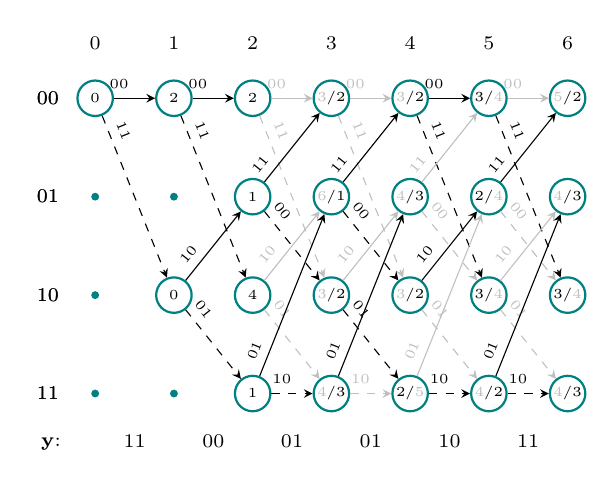
\begin{tikzpicture}[>=stealth, font=\scriptsize]
\tikzstyle{state} = [draw, circle, teal, thick, text=black, minimum size=4.5mm, inner sep=0mm, font=\tiny]
\tikzstyle{freestate} = [circle, teal, fill=teal, minimum size=1mm, inner sep=0mm]

\node[state] (node00) at (0,0) {0} ; 
\node[freestate] (node10) at (0,-1.25) {} ; 
\node[freestate] (node20) at (0,-2.5) {} ; 
\node[freestate] (node30) at (0,-3.75) {} ; 

\node[state] (node01) at (1,0) {2} ; 
\node[freestate] (node11) at (1,-1.25) {} ; 
\node[state] (node21) at (1,-2.5) {0} ; 
\node[freestate] (node31) at (1,-3.75) {} ; 

\node[state] (node02) at (2,0) {2} ; 
\node[state] (node12) at (2,-1.25) {1} ; 
\node[state] (node22) at (2,-2.5) {4} ; 
\node[state] (node32) at (2,-3.75) {1} ; 

\node[state] (node03) at (3,0) {\textcolor{lightgray}{3}\textcolor{black}{/2}} ; 
\node[state] (node13) at (3,-1.25) {\textcolor{lightgray}{6}\textcolor{black}{/1}} ; 
\node[state] (node23) at (3,-2.5) {\textcolor{lightgray}{3}\textcolor{black}{/2}} ; 
\node[state] (node33) at (3,-3.75) {\textcolor{lightgray}{4}\textcolor{black}{/3}} ; 

\node[state] (node04) at (4,0) {\textcolor{lightgray}{3}\textcolor{black}{/2}} ; 
\node[state] (node14) at (4,-1.25) {\textcolor{lightgray}{4}\textcolor{black}{/3}} ; 
\node[state] (node24) at (4,-2.5) {\textcolor{lightgray}{3}\textcolor{black}{/2}} ; 
\node[state] (node34) at (4,-3.75) {2/\textcolor{lightgray}{5}} ; 

\node[state] (node05) at (5,0) {3/\textcolor{lightgray}{4}} ; 
\node[state] (node15) at (5,-1.25) {2/\textcolor{lightgray}{4}} ; 
\node[state] (node25) at (5,-2.5) {3/\textcolor{lightgray}{4}} ; 
\node[state] (node35) at (5,-3.75) {\textcolor{lightgray}{4}\textcolor{black}{/2}} ; 

\node[state] (node06) at (6,0) {\textcolor{lightgray}{5}\textcolor{black}{/2}} ; 
\node[state] (node16) at (6,-1.25) {\textcolor{lightgray}{4}\textcolor{black}{/3}} ; 
\node[state] (node26) at (6,-2.5) {3/\textcolor{lightgray}{4}} ; 
\node[state] (node36) at (6,-3.75) {\textcolor{lightgray}{4}\textcolor{black}{/3}} ; 
\node (statelabel0) [left of=node00, xshift=4mm] {00}; 
\node (statelabel1) [left of=node10, xshift=4mm] {01}; 
\node (statelabel2) [left of=node20, xshift=4mm] {10}; 
\node (statelabel3) [left of=node30, xshift=4mm] {11};

\foreach \x in {0,...,6}
	\node (timelabel\x) [above of=node0\x, yshift=-3mm] {\x};
		
\node (statelabel0) [left of=node00, xshift=4mm] {00}; 
\node (statelabel1) [left of=node10, xshift=4mm] {01}; 
\node (statelabel2) [left of=node20, xshift=4mm] {10}; 
\node (statelabel3) [left of=node30, xshift=4mm] {11};

%t=0
\draw[->] (node00) -- (node01) node [sloped, above, very near start, font=\tiny] {00};
\draw[->, dashed] (node00) -- (node21) node [sloped, above, very near start, font=\tiny] {11};

%t=1
\draw[->] (node01) -- (node02) node [sloped, above, very near start, font=\tiny] {00};
\draw[->, dashed] (node01) -- (node22) node [sloped, above, very near start, font=\tiny] {11};
\draw[->] (node21) -- (node12) node [sloped, above, near start, font=\tiny] {10};
\draw[->, dashed] (node21) -- (node32) node [sloped, above, very near start, font=\tiny] {01};

%t=2
\draw[->, lightgray] (node02) -- (node03) node [sloped, above, very near start, font=\tiny] {00};
\draw[->, dashed, lightgray] (node02) -- (node23) node [sloped, above, very near start, font=\tiny] {11};
\draw[->] (node12) -- (node03) node [sloped, above, very near start, font=\tiny] {11};
\draw[->, dashed] (node12) -- (node23) node [sloped, above, very near start, font=\tiny] {00};
\draw[->, lightgray] (node22) -- (node13) node [sloped, above, near start, font=\tiny] {10};
\draw[->, dashed, lightgray] (node22) -- (node33) node [sloped, above, very near start, font=\tiny] {01};
\draw[->] (node32) -- (node13) node [sloped, above, very near start, font=\tiny] {01};
\draw[->, dashed] (node32) -- (node33) node [sloped, above, near start, font=\tiny] {10};

%t=3
\draw[->, lightgray] (node03) -- (node04) node [sloped, above, very near start, font=\tiny] {00};
\draw[->, dashed, lightgray] (node03) -- (node24) node [sloped, above, very near start, font=\tiny] {11};
\draw[->] (node13) -- (node04) node [sloped, above, very near start, font=\tiny] {11};
\draw[->, dashed] (node13) -- (node24) node [sloped, above, very near start, font=\tiny] {00};
\draw[->, lightgray] (node23) -- (node14) node [sloped, above, near start, font=\tiny] {10};
\draw[->, dashed] (node23) -- (node34) node [sloped, above, very near start, font=\tiny] {01};
\draw[->] (node33) -- (node14) node [sloped, above, very near start, font=\tiny] {01};
\draw[->, dashed, lightgray] (node33) -- (node34) node [sloped, above, near start, font=\tiny] {10};

%t=4
\draw[->] (node04) -- (node05) node [sloped, above, very near start, font=\tiny] {00};
\draw[->, dashed] (node04) -- (node25) node [sloped, above, very near start, font=\tiny] {11};
\draw[->, lightgray] (node14) -- (node05) node [sloped, above, very near start, font=\tiny] {11};
\draw[->, dashed, lightgray] (node14) -- (node25) node [sloped, above, very near start, font=\tiny] {00};
\draw[->] (node24) -- (node15) node [sloped, above, near start, font=\tiny] {10};
\draw[->, dashed, lightgray] (node24) -- (node35) node [sloped, above, very near start, font=\tiny] {01};
\draw[->, lightgray] (node34) -- (node15) node [sloped, above, very near start, font=\tiny] {01};
\draw[->, dashed] (node34) -- (node35) node [sloped, above, near start, font=\tiny] {10};

%t=5
\draw[->, lightgray] (node05) -- (node06) node [sloped, above, very near start, font=\tiny] {00};
\draw[->, dashed] (node05) -- (node26) node [sloped, above, very near start, font=\tiny] {11};
\draw[->] (node15) -- (node06) node [sloped, above, very near start, font=\tiny] {11};
\draw[->, dashed, lightgray] (node15) -- (node26) node [sloped, above, very near start, font=\tiny] {00};
\draw[->, lightgray] (node25) -- (node16) node [sloped, above, near start, font=\tiny] {10};
\draw[->, dashed, lightgray] (node25) -- (node36) node [sloped, above, very near start, font=\tiny] {01};
\draw[->] (node35) -- (node16) node [sloped, above, very near start, font=\tiny] {01};
\draw[->, dashed] (node35) -- (node36) node [sloped, above, near start, font=\tiny] {10};

% input & output
\node (in0) at($(node30)!0.5!(node31)+(0,-.6)$) {11};
\node (in1) at($(node31)!0.5!(node32)+(0,-.6)$) {00};
\node (in2) at($(node32)!0.5!(node33)+(0,-.6)$) {01};
\node (in3) at($(node33)!0.5!(node34)+(0,-.6)$) {01};
\node (in4) at($(node34)!0.5!(node35)+(0,-.6)$) {10};
\node (in5) at($(node35)!0.5!(node36)+(0,-.6)$) {11};
\node (inlabel) at($(node30)+(-.56,-.64)$) {$\mathbf{y}$:};

%\node (out0) [below=of in0, yshift=5mm] {\textcolor{white}{1}};
%\node (out1) [below=of in1, yshift=5mm] {\textcolor{white}{1}};
%\node (out2) [below=of in2, yshift=5mm] {\textcolor{white}{0}};
%\node (out3) [below=of in3, yshift=5mm] {\textcolor{white}{1}};
%\node (out4) [below=of in4, yshift=5mm] {\textcolor{white}{0}};
%\node (out5) [below=of in5, yshift=5mm] {\textcolor{white}{0}};
%\node (outlabel) at($(node30)+(-.6,-1.53)$) {\textcolor{white}{$\mathbf{u'}$:}};

\end{tikzpicture}
			}
			\caption{}
			\label{abb:trellis_dek_hard_a}
		\end{subfigure}
		\begin{subfigure}[t]{0.42\textwidth}
			\centering
			\resizebox{0.99\textwidth}{!}{%
				% trellis_dekodierung_hard2.tex
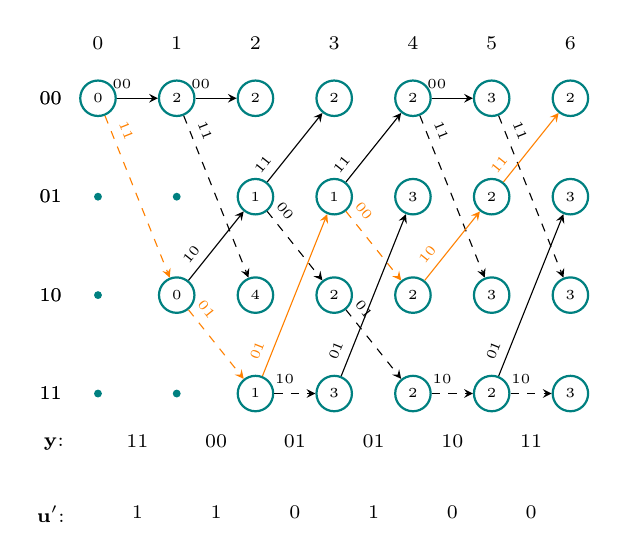
\begin{tikzpicture}[>=stealth, font=\scriptsize]
\tikzstyle{state} = [draw, circle, teal, thick, text=black, minimum size=4.5mm, inner sep=0mm, font=\tiny]
\tikzstyle{freestate} = [circle, teal, fill=teal, minimum size=1mm, inner sep=0mm]

\node[state] (node00) at (0,0) {0} ; 
\node[freestate] (node10) at (0,-1.25) {} ; 
\node[freestate] (node20) at (0,-2.5) {} ; 
\node[freestate] (node30) at (0,-3.75) {} ; 

\node[state] (node01) at (1,0) {2} ; 
\node[freestate] (node11) at (1,-1.25) {} ; 
\node[state] (node21) at (1,-2.5) {0} ; 
\node[freestate] (node31) at (1,-3.75) {} ; 

\node[state] (node02) at (2,0) {2} ; 
\node[state] (node12) at (2,-1.25) {1} ; 
\node[state] (node22) at (2,-2.5) {4} ; 
\node[state] (node32) at (2,-3.75) {1} ; 

\node[state] (node03) at (3,0) {2} ; 
\node[state] (node13) at (3,-1.25) {1} ; 
\node[state] (node23) at (3,-2.5) {2} ; 
\node[state] (node33) at (3,-3.75) {3} ; 

\node[state] (node04) at (4,0) {2} ; 
\node[state] (node14) at (4,-1.25) {3} ; 
\node[state] (node24) at (4,-2.5) {2} ; 
\node[state] (node34) at (4,-3.75) {2} ; 

\node[state] (node05) at (5,0) {3} ; 
\node[state] (node15) at (5,-1.25) {2} ; 
\node[state] (node25) at (5,-2.5) {3} ; 
\node[state] (node35) at (5,-3.75) {2} ; 

\node[state] (node06) at (6,0) {2} ; 
\node[state] (node16) at (6,-1.25) {3} ; 
\node[state] (node26) at (6,-2.5) {3} ; 
\node[state] (node36) at (6,-3.75) {3} ; 
\node (statelabel0) [left of=node00, xshift=4mm] {00}; 
\node (statelabel1) [left of=node10, xshift=4mm] {01}; 
\node (statelabel2) [left of=node20, xshift=4mm] {10}; 
\node (statelabel3) [left of=node30, xshift=4mm] {11};

\foreach \x in {0,...,6}
	\node (timelabel\x) [above of=node0\x, yshift=-3mm] {\x};
		
\node (statelabel0) [left of=node00, xshift=4mm] {00}; 
\node (statelabel1) [left of=node10, xshift=4mm] {01}; 
\node (statelabel2) [left of=node20, xshift=4mm] {10}; 
\node (statelabel3) [left of=node30, xshift=4mm] {11};

%t=0
\draw[->] (node00) -- (node01) node [sloped, above, very near start, font=\tiny] {00};
\draw[->, dashed, orange] (node00) -- (node21) node [sloped, above, very near start, font=\tiny] {11};

%t=1
\draw[->] (node01) -- (node02) node [sloped, above, very near start, font=\tiny] {00};
\draw[->, dashed] (node01) -- (node22) node [sloped, above, very near start, font=\tiny] {11};
\draw[->] (node21) -- (node12) node [sloped, above, near start, font=\tiny] {10};
\draw[->, dashed, orange] (node21) -- (node32) node [sloped, above, very near start, font=\tiny] {01};

%t=2
%\draw[->, lightgray] (node02) -- (node03) node [sloped, above, very near start, font=\tiny] {00};
%\draw[->, dashed, lightgray] (node02) -- (node23) node [sloped, above, very near start, font=\tiny] {11};
\draw[->] (node12) -- (node03) node [sloped, above, very near start, font=\tiny] {11};
\draw[->, dashed] (node12) -- (node23) node [sloped, above, very near start, font=\tiny] {00};
%\draw[->, lightgray] (node22) -- (node13) node [sloped, above, near start, font=\tiny] {10};
%\draw[->, dashed, lightgray] (node22) -- (node33) node [sloped, above, very near start, font=\tiny] {01};
\draw[->, orange] (node32) -- (node13) node [sloped, above, very near start, font=\tiny] {01};
\draw[->, dashed] (node32) -- (node33) node [sloped, above, near start, font=\tiny] {10};

%t=3
%\draw[->, lightgray] (node03) -- (node04) node [sloped, above, very near start, font=\tiny] {00};
%\draw[->, dashed, lightgray] (node03) -- (node24) node [sloped, above, very near start, font=\tiny] {11};
\draw[->] (node13) -- (node04) node [sloped, above, very near start, font=\tiny] {11};
\draw[->, dashed, orange] (node13) -- (node24) node [sloped, above, very near start, font=\tiny] {00};
%\draw[->, lightgray] (node23) -- (node14) node [sloped, above, near start, font=\tiny] {10};
\draw[->, dashed] (node23) -- (node34) node [sloped, above, very near start, font=\tiny] {01};
\draw[->] (node33) -- (node14) node [sloped, above, very near start, font=\tiny] {01};
%\draw[->, dashed, lightgray] (node33) -- (node34) node [sloped, above, near start, font=\tiny] {10};

%t=4
\draw[->] (node04) -- (node05) node [sloped, above, very near start, font=\tiny] {00};
\draw[->, dashed] (node04) -- (node25) node [sloped, above, very near start, font=\tiny] {11};
%\draw[->, lightgray] (node14) -- (node05) node [sloped, above, very near start, font=\tiny] {11};
%\draw[->, dashed, lightgray] (node14) -- (node25) node [sloped, above, very near start, font=\tiny] {00};
\draw[->,orange] (node24) -- (node15) node [sloped, above, near start, font=\tiny] {10};
%\draw[->, dashed, lightgray] (node24) -- (node35) node [sloped, above, very near start, font=\tiny] {01};
%\draw[->, lightgray] (node34) -- (node15) node [sloped, above, very near start, font=\tiny] {01};
\draw[->, dashed] (node34) -- (node35) node [sloped, above, near start, font=\tiny] {10};

%t=5
%\draw[->, lightgray] (node05) -- (node06) node [sloped, above, very near start, font=\tiny] {00};
\draw[->, dashed] (node05) -- (node26) node [sloped, above, very near start, font=\tiny] {11};
\draw[->,orange] (node15) -- (node06) node [sloped, above, very near start, font=\tiny] {11};
%\draw[->, dashed, lightgray] (node15) -- (node26) node [sloped, above, very near start, font=\tiny] {00};
%\draw[->, lightgray] (node25) -- (node16) node [sloped, above, near start, font=\tiny] {10};
%\draw[->, dashed, lightgray] (node25) -- (node36) node [sloped, above, very near start, font=\tiny] {01};
\draw[->] (node35) -- (node16) node [sloped, above, very near start, font=\tiny] {01};
\draw[->, dashed] (node35) -- (node36) node [sloped, above, near start, font=\tiny] {10};

% input & output
\node (in0) at($(node30)!0.5!(node31)+(0,-.6)$) {11};
\node (in1) at($(node31)!0.5!(node32)+(0,-.6)$) {00};
\node (in2) at($(node32)!0.5!(node33)+(0,-.6)$) {01};
\node (in3) at($(node33)!0.5!(node34)+(0,-.6)$) {01};
\node (in4) at($(node34)!0.5!(node35)+(0,-.6)$) {10};
\node (in5) at($(node35)!0.5!(node36)+(0,-.6)$) {11};
\node (inlabel) at($(node30)+(-.56,-.64)$) {$\mathbf{y}$:};

\node (out0) [below=of in0, yshift=5mm] {1};
\node (out1) [below=of in1, yshift=5mm] {1};
\node (out2) [below=of in2, yshift=5mm] {0};
\node (out3) [below=of in3, yshift=5mm] {1};
\node (out4) [below=of in4, yshift=5mm] {0};
\node (out5) [below=of in5, yshift=5mm] {0};
\node (outlabel) at($(node30)+(-.6,-1.53)$) {$\mathbf{u'}$:};

\end{tikzpicture}
			}
			\caption{}
			\label{abb:trellis_dek_hard_b}
		\end{subfigure}
	}
	\caption{Trellis der hard decision Dekodierung aus Beispiel~\ref{bsp:B3}.}
	\label{abb:trellis_dekodierung_hard}
\end{figure}

\subsubsection{soft decision}
\label{kapitel:grundlagen_soft_decision}
Vor der Übertragung eines Kodeworts werden die Kodebits 0 bzw. 1 nach Gleichung~\eqref{eq:bit_zu_signal_abbildung} auf die Signalzustände +1 bzw. -1 abgebildet. Bei der hard decision Dekodierung wird vor der Dekodierung das Signal nach Gleichung~\eqref{eq:signal_zu_bit_abbildung} wieder zu einem Bitvektor zurück umgewandelt. Die soft decision Dekodierung lässt diese Rücktransformation aus und verwendet die exakten Signalpegel. Dadurch erzielt die soft decision Dekodierung eine noch bessere Fehlerkorrektur. Die Metrik für eine Kante, die einen Zustand $s$ zum Zeitpunkt $t$ mit einem Zustand $s'$ zum Zeitpunkt $t+1$ verbindet, entspricht dem Skalarprodukt der Signalzustände der Bewertung der Kante zwischen $s$ und $s'$ und dem zum Zeitpunkt $t$ empfangenen Teil des Signals. Der Viterbi-Algorithmus funktioniert analog zur soft decision Dekodierung, jedoch wird der Pfad mit der maximal Metrix gesucht. Treffen zwei Pfade aufeinander, wird der Pfad mit der kleineren Metrik verworfen. Das Backtracking beginnt hier bei der größten Metrik. Als Ergebnis resultiert die Nachricht, dessen Signal das größte Skalarprodukt mit dem empfangenen Signal hat.
\\
\\
Die Nachricht wird mittels \emph{Soft-Werten} und \emph{Hard-Werten} angegeben. Die Soft-Werte geben neben der dekodierten Nachricht die Zuverlässigkeitswerte für die Bits an, d.h. mit welcher Wahrscheinlichkeit das Bit mit dem tatsächlich gesendeten Bit der Quellnachricht übereinstimmt. Positive Soft-Werte werden auf eine 0, negative auf eine 1 abgebildet. Der Betrag des Soft-Wertes gibt die Zuverlässigkeit an, wobei gilt, je höher der Betrag, desto zuverlässiger das dekodierte Bit. Die Hard-Werte entsprechen der Abbildung der Soft-Werte auf die Bit-Werte 0 bzw. 1. Der Viterbi-Algorithmus mit Soft-Werten wird auch SOVA (Soft Output Viterbi Algorithm) genannt. Die Berechnung der Soft-Werte ist in \cite[S. 228 ff.]{schonfeld2012informations} beschrieben.

\begin{beispiel}
Gegeben sei der Faltungskodierer aus Beispiel~\ref{bsp:B1} und ein empfangenes Signal $\mathbf{y}=\left( -1~-1~~0.5~-1~~0.9~-0.9~~1~-0.2~~-0.8~-0.1~-1~-1\right)$ welches durch Rauschen verfälscht wurde und dekodiert werden soll. Abbildung~ \ref{abb:trellis_dekodierung_soft} zeigt die Dekodierung im Trellis. Abbildung~\ref{abb:trellis_dek_soft_a} zeigt die Metriken aller Pfade. Die verworfenen Pfade sind grau dargestellt. Beispielsweise ergibt sich die Metrik zum Zeitpunkt 1 im Zustand 00 durch $0+\left( 1\cdot\left( -1\right) + 1\cdot\left( -1\right)\right) =0-2=-2$, im Zustand 10 durch $0+\left( \left( -1\right)\cdot\left( -1\right) + \left( -1\right)\cdot\left( -1\right)\right) =0+2=2$. Der erste Summand entspricht der Metrik des vorigen Zustands. Die Bits der Kantenbewertung im Trellis müssen für die Berechnung des Skalarprodukts auf die Signalzustände +1 bzw. -1 abgebildet werden. In Abbildung~\ref{abb:trellis_dek_soft_b} werden die verworfenen Pfade nicht mehr angezeigt. Durch Backtracking erhält man die dekodierte Nachricht $\mathbf{u'}=\left( 110100\right)$. Der resultierende Pfad ist orange hervorgehoben.
\label{bsp:B4}
\end{beispiel}

\begin{figure}[t]
	\centering
	\resizebox{\textwidth}{!}{%
		\begin{subfigure}[t]{0.42\textwidth}
			\centering
			\resizebox{0.99\textwidth}{!}{%
				% trellis_dekodierung_soft1.tex
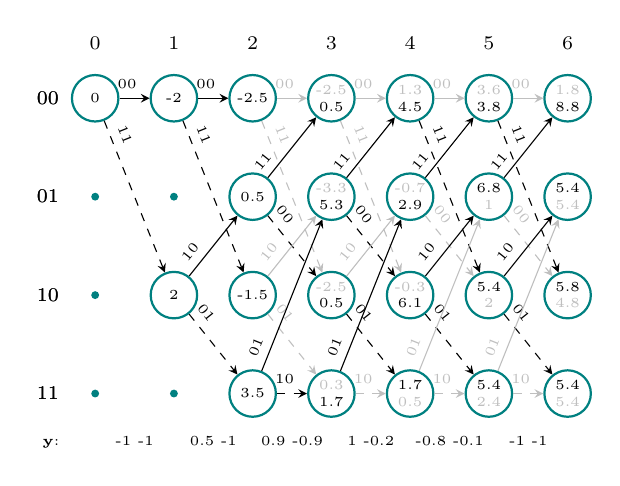
\begin{tikzpicture}[>=stealth, font=\scriptsize]
\tikzstyle{state} = [draw, circle, teal, thick, text=black, minimum size=5.9mm, inner sep=0mm, font=\tiny, align=center]
\tikzstyle{freestate} = [circle, teal, fill=teal, minimum size=1mm, inner sep=0mm]

\node[state] (node00) at (0,0) {0} ; 
\node[freestate] (node10) at (0,-1.25) {} ; 
\node[freestate] (node20) at (0,-2.5) {} ; 
\node[freestate] (node30) at (0,-3.75) {} ; 

\node[state] (node01) at (1,0) {-2} ; 
\node[freestate] (node11) at (1,-1.25) {} ; 
\node[state] (node21) at (1,-2.5) {2} ; 
\node[freestate] (node31) at (1,-3.75) {} ; 

\node[state] (node02) at (2,0) {-2.5} ; 
\node[state] (node12) at (2,-1.25) {0.5} ; 
\node[state] (node22) at (2,-2.5) {-1.5} ; 
\node[state] (node32) at (2,-3.75) {3.5} ; 

\node[state] (node03) at (3,0) {\textcolor{lightgray}{-2.5}\\ \textcolor{black}{0.5}} ; 
\node[state] (node13) at (3,-1.25) {\textcolor{lightgray}{-3.3}\\ \textcolor{black}{5.3}} ; 
\node[state] (node23) at (3,-2.5) {\textcolor{lightgray}{-2.5}\\ \textcolor{black}{0.5}} ; 
\node[state] (node33) at (3,-3.75) {\textcolor{lightgray}{0.3}\\ \textcolor{black}{1.7}} ; 

\node[state] (node04) at (4,0) {\textcolor{lightgray}{1.3}\\ \textcolor{black}{4.5}} ; 
\node[state] (node14) at (4,-1.25) {\textcolor{lightgray}{-0.7}\\ \textcolor{black}{2.9}} ; 
\node[state] (node24) at (4,-2.5) {\textcolor{lightgray}{-0.3}\\ \textcolor{black}{6.1}} ; 
\node[state] (node34) at (4,-3.75) {1.7\\ \textcolor{lightgray}{0.5}} ; 

\node[state] (node05) at (5,0) {\textcolor{lightgray}{3.6}\\ \textcolor{black}{3.8}} ; 
\node[state] (node15) at (5,-1.25) {6.8\\ \textcolor{lightgray}{1}} ; 
\node[state] (node25) at (5,-2.5) {5.4\\ \textcolor{lightgray}{2}} ; 
\node[state] (node35) at (5,-3.75) {5.4\\ \textcolor{lightgray}{2.4}} ; 

\node[state] (node06) at (6,0) {\textcolor{lightgray}{1.8}\\ \textcolor{black}{8.8}} ; 
\node[state] (node16) at (6,-1.25) {5.4\\ \textcolor{lightgray}{5.4}} ; 
\node[state] (node26) at (6,-2.5) {5.8\\ \textcolor{lightgray}{4.8}} ; 
\node[state] (node36) at (6,-3.75) {5.4\\ \textcolor{lightgray}{5.4}} ; 
\node (statelabel0) [left of=node00, xshift=4mm] {00}; 
\node (statelabel1) [left of=node10, xshift=4mm] {01}; 
\node (statelabel2) [left of=node20, xshift=4mm] {10}; 
\node (statelabel3) [left of=node30, xshift=4mm] {11};

\foreach \x in {0,...,6}
	\node (timelabel\x) [above of=node0\x, yshift=-3mm] {\x};
		
\node (statelabel0) [left of=node00, xshift=4mm] {00}; 
\node (statelabel1) [left of=node10, xshift=4mm] {01}; 
\node (statelabel2) [left of=node20, xshift=4mm] {10}; 
\node (statelabel3) [left of=node30, xshift=4mm] {11};

%t=0
\draw[->] (node00) -- (node01) node [sloped, above, near start, font=\tiny] {00};
\draw[->, dashed] (node00) -- (node21) node [sloped, above, very near start, font=\tiny] {11};

%t=1
\draw[->] (node01) -- (node02) node [sloped, above, near start, font=\tiny] {00};
\draw[->, dashed] (node01) -- (node22) node [sloped, above, very near start, font=\tiny] {11};
\draw[->] (node21) -- (node12) node [sloped, above, near start, font=\tiny] {10};
\draw[->, dashed] (node21) -- (node32) node [sloped, above, very near start, font=\tiny] {01};

%t=2
\draw[->, lightgray] (node02) -- (node03) node [sloped, above, near start, font=\tiny] {00};
\draw[->, dashed, lightgray] (node02) -- (node23) node [sloped, above, very near start, font=\tiny] {11};
\draw[->] (node12) -- (node03) node [sloped, above, very near start, font=\tiny] {11};
\draw[->, dashed] (node12) -- (node23) node [sloped, above, very near start, font=\tiny] {00};
\draw[->, lightgray] (node22) -- (node13) node [sloped, above, near start, font=\tiny] {10};
\draw[->, dashed, lightgray] (node22) -- (node33) node [sloped, above, very near start, font=\tiny] {01};
\draw[->] (node32) -- (node13) node [sloped, above, very near start, font=\tiny] {01};
\draw[->, dashed] (node32) -- (node33) node [sloped, above, near start, font=\tiny] {10};

%t=3
\draw[->, lightgray] (node03) -- (node04) node [sloped, above, near start, font=\tiny] {00};
\draw[->, dashed, lightgray] (node03) -- (node24) node [sloped, above, very near start, font=\tiny] {11};
\draw[->] (node13) -- (node04) node [sloped, above, very near start, font=\tiny] {11};
\draw[->, dashed] (node13) -- (node24) node [sloped, above, very near start, font=\tiny] {00};
\draw[->, lightgray] (node23) -- (node14) node [sloped, above, near start, font=\tiny] {10};
\draw[->, dashed] (node23) -- (node34) node [sloped, above, very near start, font=\tiny] {01};
\draw[->] (node33) -- (node14) node [sloped, above, very near start, font=\tiny] {01};
\draw[->, dashed, lightgray] (node33) -- (node34) node [sloped, above, near start, font=\tiny] {10};

%t=4
\draw[->, lightgray] (node04) -- (node05) node [sloped, above, near start, font=\tiny] {00};
\draw[->, dashed] (node04) -- (node25) node [sloped, above, very near start, font=\tiny] {11};
\draw[->] (node14) -- (node05) node [sloped, above, very near start, font=\tiny] {11};
\draw[->, dashed, lightgray] (node14) -- (node25) node [sloped, above, very near start, font=\tiny] {00};
\draw[->] (node24) -- (node15) node [sloped, above, near start, font=\tiny] {10};
\draw[->, dashed] (node24) -- (node35) node [sloped, above, very near start, font=\tiny] {01};
\draw[->, lightgray] (node34) -- (node15) node [sloped, above, very near start, font=\tiny] {01};
\draw[->, dashed, lightgray] (node34) -- (node35) node [sloped, above, near start, font=\tiny] {10};

%t=5
\draw[->, lightgray] (node05) -- (node06) node [sloped, above, near start, font=\tiny] {00};
\draw[->, dashed] (node05) -- (node26) node [sloped, above, very near start, font=\tiny] {11};
\draw[->] (node15) -- (node06) node [sloped, above, very near start, font=\tiny] {11};
\draw[->, dashed, lightgray] (node15) -- (node26) node [sloped, above, very near start, font=\tiny] {00};
\draw[->] (node25) -- (node16) node [sloped, above, near start, font=\tiny] {10};
\draw[->, dashed] (node25) -- (node36) node [sloped, above, very near start, font=\tiny] {01};
\draw[->, lightgray] (node35) -- (node16) node [sloped, above, very near start, font=\tiny] {01};
\draw[->, dashed, lightgray] (node35) -- (node36) node [sloped, above, near start, font=\tiny] {10};

% input & output
\node[font=\tiny] (in0) at($(node30)!0.5!(node31)+(0,-.6)$) {-1~-1};
\node[font=\tiny] (in1) at($(node31)!0.5!(node32)+(0,-.6)$) {0.5~-1};
\node[font=\tiny] (in2) at($(node32)!0.5!(node33)+(0,-.6)$) {0.9~-0.9};
\node[font=\tiny] (in3) at($(node33)!0.5!(node34)+(0,-.6)$) {1~-0.2};
\node[font=\tiny] (in4) at($(node34)!0.5!(node35)+(0,-.6)$) {-0.8~-0.1};
\node[font=\tiny] (in5) at($(node35)!0.5!(node36)+(0,-.6)$) {-1~-1};
\node[font=\tiny] (inlabel) at($(node30)+(-.56,-.64)$) {$\mathbf{y}$:};

%\node[font=\tiny] (out0) [below=of in0, yshift=5mm] {\textcolor{white}{-4.3}};
%\node[font=\tiny] (out1) [below=of in1, yshift=5mm] {\textcolor{white}{-2.9}};
%\node[font=\tiny] (out2) [below=of in2, yshift=5mm] {\textcolor{white}{2.9}};
%\node[font=\tiny] (out3) [below=of in3, yshift=5mm] {\textcolor{white}{-2.9}};
%\node[font=\tiny] (out4) [below=of in4, yshift=5mm] {\textcolor{white}{2.9}};
%\node[font=\tiny] (out5) [below=of in5, yshift=5mm] {\textcolor{white}{3.5}};
%\node[font=\tiny] (outlabel) at($(node30)+(-.65,-1.53)$) {\textcolor{white}{$\mathbf{u'_{s}}$:}};
%
%\node[font=\tiny] [below=of out0, yshift=5mm] {\textcolor{white}{1}};
%\node[font=\tiny] [below=of out1, yshift=5mm] {\textcolor{white}{1}};
%\node[font=\tiny] [below=of out2, yshift=5mm] {\textcolor{white}{0}};
%\node[font=\tiny] [below=of out3, yshift=5mm] {\textcolor{white}{1}};
%\node[font=\tiny] [below=of out4, yshift=5mm] {\textcolor{white}{0}};
%\node[font=\tiny] [below=of out5, yshift=5mm] {\textcolor{white}{0}};
%\node[font=\tiny] at($(node30)+(-.65,-2.43)$) {\textcolor{white}{$\mathbf{u'_{h}}$:}};

\end{tikzpicture}
			}
			\caption{}
			\label{abb:trellis_dek_soft_a}
		\end{subfigure}
		\begin{subfigure}[t]{0.42\textwidth}
			\centering
			\resizebox{0.99\textwidth}{!}{%
				% trellis_dekodierung_soft2.tex
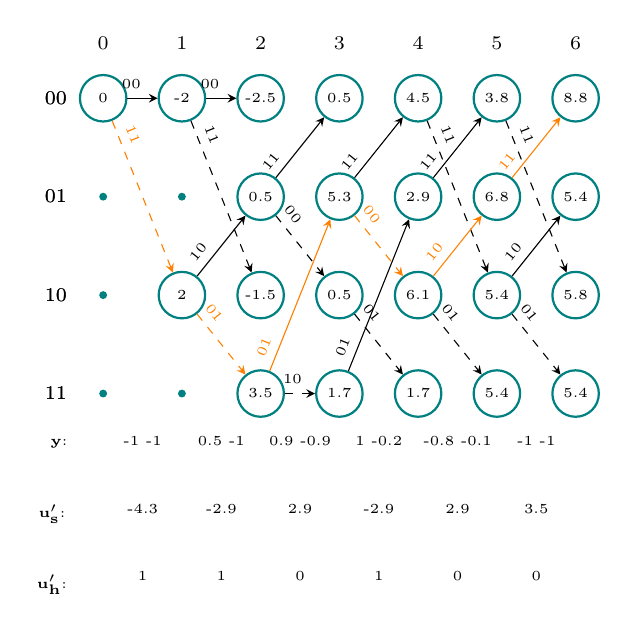
\begin{tikzpicture}[>=stealth, font=\scriptsize]
\tikzstyle{state} = [draw, circle, teal, thick, text=black, minimum size=5.9mm, inner sep=0mm, font=\tiny]
\tikzstyle{freestate} = [circle, teal, fill=teal, minimum size=1mm, inner sep=0mm]

\node[state] (node00) at (0,0) {0} ; 
\node[freestate] (node10) at (0,-1.25) {} ; 
\node[freestate] (node20) at (0,-2.5) {} ; 
\node[freestate] (node30) at (0,-3.75) {} ; 

\node[state, font=\tiny] (node01) at (1,0) {-2} ; 
\node[freestate] (node11) at (1,-1.25) {} ; 
\node[state] (node21) at (1,-2.5) {2} ; 
\node[freestate] (node31) at (1,-3.75) {} ; 

\node[state, ] (node02) at (2,0) {-2.5} ; 
\node[state] (node12) at (2,-1.25) {0.5} ; 
\node[state] (node22) at (2,-2.5) {-1.5} ; 
\node[state] (node32) at (2,-3.75) {3.5} ; 

\node[state] (node03) at (3,0) {0.5} ; 
\node[state] (node13) at (3,-1.25) {5.3} ; 
\node[state] (node23) at (3,-2.5) {0.5} ; 
\node[state] (node33) at (3,-3.75) {1.7} ; 

\node[state] (node04) at (4,0) {4.5} ; 
\node[state] (node14) at (4,-1.25) {2.9} ; 
\node[state] (node24) at (4,-2.5) {6.1} ; 
\node[state] (node34) at (4,-3.75) {1.7} ; 

\node[state] (node05) at (5,0) {3.8} ; 
\node[state] (node15) at (5,-1.25) {6.8} ; 
\node[state] (node25) at (5,-2.5) {5.4} ; 
\node[state] (node35) at (5,-3.75) {5.4} ; 

\node[state] (node06) at (6,0) {8.8} ; 
\node[state] (node16) at (6,-1.25) {5.4} ; 
\node[state] (node26) at (6,-2.5) {5.8} ; 
\node[state] (node36) at (6,-3.75) {5.4} ; 
\node (statelabel0) [left of=node00, xshift=4mm] {00}; 
\node (statelabel1) [left of=node10, xshift=4mm] {01}; 
\node (statelabel2) [left of=node20, xshift=4mm] {10}; 
\node (statelabel3) [left of=node30, xshift=4mm] {11};

\foreach \x in {0,...,6}
	\node (timelabel\x) [above of=node0\x, yshift=-3mm] {\x};
		
\node (statelabel0) [left of=node00, xshift=4mm] {00}; 
\node (statelabel1) [left of=node10, xshift=4mm] {01}; 
\node (statelabel2) [left of=node20, xshift=4mm] {10}; 
\node (statelabel3) [left of=node30, xshift=4mm] {11};

%t=0
\draw[->] (node00) -- (node01) node [sloped, above, very near start, font=\tiny] {00};
\draw[->, dashed, orange] (node00) -- (node21) node [sloped, above, very near start, font=\tiny] {11};

%t=1
\draw[->] (node01) -- (node02) node [sloped, above, very near start, font=\tiny] {00};
\draw[->, dashed] (node01) -- (node22) node [sloped, above, very near start, font=\tiny] {11};
\draw[->] (node21) -- (node12) node [sloped, above, near start, font=\tiny] {10};
\draw[->, dashed, orange] (node21) -- (node32) node [sloped, above, very near start, font=\tiny] {01};

%t=2
%\draw[->, lightgray] (node02) -- (node03) node [sloped, above, very near start, font=\tiny] {00};
%\draw[->, dashed, lightgray] (node02) -- (node23) node [sloped, above, very near start, font=\tiny] {11};
\draw[->] (node12) -- (node03) node [sloped, above, very near start, font=\tiny] {11};
\draw[->, dashed] (node12) -- (node23) node [sloped, above, very near start, font=\tiny] {00};
%\draw[->, lightgray] (node22) -- (node13) node [sloped, above, near start, font=\tiny] {10};
%\draw[->, dashed, lightgray] (node22) -- (node33) node [sloped, above, very near start, font=\tiny] {01};
\draw[->, orange] (node32) -- (node13) node [sloped, above, very near start, font=\tiny] {01};
\draw[->, dashed] (node32) -- (node33) node [sloped, above, near start, font=\tiny] {10};

%t=3
%\draw[->, lightgray] (node03) -- (node04) node [sloped, above, very near start, font=\tiny] {00};
%\draw[->, dashed, lightgray] (node03) -- (node24) node [sloped, above, very near start, font=\tiny] {11};
\draw[->] (node13) -- (node04) node [sloped, above, very near start, font=\tiny] {11};
\draw[->, dashed, orange] (node13) -- (node24) node [sloped, above, very near start, font=\tiny] {00};
%\draw[->, lightgray] (node23) -- (node14) node [sloped, above, near start, font=\tiny] {10};
\draw[->, dashed] (node23) -- (node34) node [sloped, above, very near start, font=\tiny] {01};
\draw[->] (node33) -- (node14) node [sloped, above, very near start, font=\tiny] {01};
%\draw[->, dashed, lightgray] (node33) -- (node34) node [sloped, above, near start, font=\tiny] {10};

%t=4
%\draw[->, lightgray] (node04) -- (node05) node [sloped, above, very near start, font=\tiny] {00};
\draw[->, dashed] (node04) -- (node25) node [sloped, above, very near start, font=\tiny] {11};
\draw[->] (node14) -- (node05) node [sloped, above, very near start, font=\tiny] {11};
%\draw[->, dashed, lightgray] (node14) -- (node25) node [sloped, above, very near start, font=\tiny] {00};
\draw[->, orange] (node24) -- (node15) node [sloped, above, near start, font=\tiny] {10};
\draw[->, dashed] (node24) -- (node35) node [sloped, above, very near start, font=\tiny] {01};
%\draw[->, lightgray] (node34) -- (node15) node [sloped, above, very near start, font=\tiny] {01};
%\draw[->, dashed, lightgray] (node34) -- (node35) node [sloped, above, near start, font=\tiny] {10};

%t=5
%\draw[->, lightgray] (node05) -- (node06) node [sloped, above, very near start, font=\tiny] {00};
\draw[->, dashed] (node05) -- (node26) node [sloped, above, very near start, font=\tiny] {11};
\draw[->, orange] (node15) -- (node06) node [sloped, above, very near start, font=\tiny] {11};
%\draw[->, dashed, lightgray] (node15) -- (node26) node [sloped, above, very near start, font=\tiny] {00};
\draw[->] (node25) -- (node16) node [sloped, above, near start, font=\tiny] {10};
\draw[->, dashed] (node25) -- (node36) node [sloped, above, very near start, font=\tiny] {01};
%\draw[->, lightgray] (node35) -- (node16) node [sloped, above, very near start, font=\tiny] {01};
%\draw[->, dashed, lightgray] (node35) -- (node36) node [sloped, above, near start, font=\tiny] {10};

% input & output
\node[font=\tiny] (in0) at($(node30)!0.5!(node31)+(0,-.6)$) {-1~-1};
\node[font=\tiny] (in1) at($(node31)!0.5!(node32)+(0,-.6)$) {0.5~-1};
\node[font=\tiny] (in2) at($(node32)!0.5!(node33)+(0,-.6)$) {0.9~-0.9};
\node[font=\tiny] (in3) at($(node33)!0.5!(node34)+(0,-.6)$) {1~-0.2};
\node[font=\tiny] (in4) at($(node34)!0.5!(node35)+(0,-.6)$) {-0.8~-0.1};
\node[font=\tiny] (in5) at($(node35)!0.5!(node36)+(0,-.6)$) {-1~-1};
\node[font=\tiny] (inlabel) at($(node30)+(-.56,-.64)$) {$\mathbf{y}$:};

\node[font=\tiny] (out0) [below=of in0, yshift=5mm] {-4.3};
\node[font=\tiny] (out1) [below=of in1, yshift=5mm] {-2.9};
\node[font=\tiny] (out2) [below=of in2, yshift=5mm] {2.9};
\node[font=\tiny] (out3) [below=of in3, yshift=5mm] {-2.9};
\node[font=\tiny] (out4) [below=of in4, yshift=5mm] {2.9};
\node[font=\tiny] (out5) [below=of in5, yshift=5mm] {3.5};
\node[font=\tiny] (outlabel) at($(node30)+(-.65,-1.53)$) {$\mathbf{u'_{s}}$:};

\node[font=\tiny] [below=of out0, yshift=5mm] {1};
\node[font=\tiny] [below=of out1, yshift=5mm] {1};
\node[font=\tiny] [below=of out2, yshift=5mm] {0};
\node[font=\tiny] [below=of out3, yshift=5mm] {1};
\node[font=\tiny] [below=of out4, yshift=5mm] {0};
\node[font=\tiny] [below=of out5, yshift=5mm] {0};
\node[font=\tiny] at($(node30)+(-.65,-2.43)$) {$\mathbf{u'_{h}}$:};

\end{tikzpicture}
			}
			\caption{}
			\label{abb:trellis_dek_soft_b}
		\end{subfigure}
	}
	\caption{Trellis der soft decision Dekodierung aus Beispiel~\ref{bsp:B4}.}
	\label{abb:trellis_dekodierung_soft}
\end{figure}

\subsection{Katastrophale Faltungskodierer}
\label{kapitel:grundlagen_katastrophale_kodierer}
Sei $\mathbf{u}$ eine Nachricht, die mit den Generatorpolynomen in $G$ zum Kode $\mathbf{v}$ kodiert wird. Nach der Übertragung erhält der Dekodierer den Kode $\mathbf{y}$, der aufgrund von Rauschen verändert sein könnte. Der Dekodierer findet ein Kodewort $\mathbf{v'}$ welches $\mathbf{v}$ am nächsten ist. Aus $\mathbf{v'}$ kann die Schätzung $\mathbf{u'}$ berechnet werden, die möglichst $\mathbf{u}$ entspricht. Dies ist bei einer fehlerfreien Übertragung, d.h. $\mathbf{v'}=\mathbf{v}$, sicherlich der Fall. Zu untersuchen ist der Fall $\mathbf{v'}\neq\mathbf{v}$:\\
Zu erwarten wäre, wenn sich $\mathbf{v'}$ und $\mathbf{v}$ in endlich vielen Stellen unterscheiden, dass sich auch $\mathbf{u'}$ und $\mathbf{u}$ in endlich vielen Stellen unterscheiden. Wenn sich $\mathbf{u'}$ und $\mathbf{u}$ in unendlich vielen Stellen unterscheiden wäre das \enquote{katastrophal}. Ein Faltungskodierer wird katastrophal genannt, wenn es eine Nachricht mit unendlichem Hamming-Gewicht gibt, sodass sein Kode endliches Hamming-Gewicht hat. Katastrophale Kodierer sind zu vermeiden, da eine endliche Anzahl an Übertragungsfehler zu einer unendlichen Anzahl an Dekodierfehler führen kann. \cite[S. 569]{huffman2010fundamentals}
\\
\\
Zur Überprüfung, ob ein Kodierer katastrophal ist, hilft das Theorem von Massey-Sain~\cite[S. 570]{huffman2010fundamentals}. Gegeben ein Faltungskodierer mit einem Eingang und der Generatormatrix $G$ als Polynome über $D$, so ist der Faltungskodierer nicht katastrophal genau dann, wenn der größte gemeinsame Teiler der Generatorpolynome eine Potenz von $D$ ist.
\begin{figure}[t]
	\centering
	\begin{subfigure}{0.45\textwidth}
		\centering
		\resizebox{0.90\textwidth}{!}{%
			% systematischer_kodierer.tex
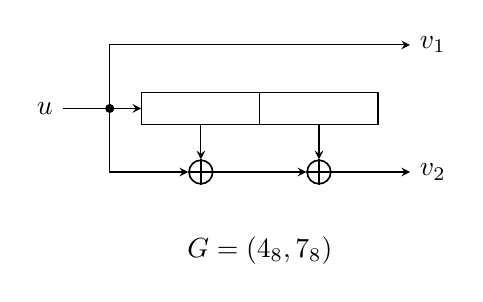
\begin{tikzpicture}[>=stealth]
\tikzstyle{rect} = [draw, rectangle, minimum width=30mm, inner sep=0mm, minimum height=4mm]
\tikzstyle{xor} = [draw, circle, semithick, minimum size=3mm, inner sep=0mm]

\node[rect] (rect) {};
\draw[-] (rect.north) -- (rect.south);
\draw[<-] (rect.west) -- ++(-10mm,0) node [left] {$u$};

\draw[->] ($(rect.west)+(-4mm,0)$) |- ($(rect.north east)+(4mm,6mm)$) node [right] {$v_{1}$};

\node[xor] (xor1) at ($(rect.south)+(-7.5mm,-6mm)$) {};
\draw[semithick] (xor1.north) -- (xor1.south);
\draw[semithick] (xor1.west) -- (xor1.east);
\draw[->] ($(rect.south)+(-7.5mm,0)$) -- (xor1.north);

\node[xor] (xor2) at ($(rect.south)+(7.5mm,-6mm)$) {};
\draw[semithick] (xor2.north) -- (xor2.south);
\draw[semithick] (xor2.west) -- (xor2.east);
\draw[->] ($(rect.south)+(7.5mm,0)$) -- (xor2.north);

\draw[->] ($(rect.west)+(-4mm,0)$) |- (xor1.west);
\draw[->] (xor1.east) -- (xor2.west);
\draw[->] (xor2.east) -- ($(rect.south east)+(4mm,-6mm)$) node [right] {$v_{2}$};
\draw[black, fill=black] ($(rect.west)+(-4mm,0)$) circle [radius=.5mm];

\node at ($(rect.south)+(0,-16mm)$) {$G=\left( 4_{8},7_{8}\right)$};
\end{tikzpicture}
		}
		\caption{Systematischer Faltungskodierer}
		\label{abb:systematischer_kodierer}
	\end{subfigure}
	~ % spacing between subfigures
	\begin{subfigure}{0.45\textwidth}
		\centering
		\resizebox{0.99\textwidth}{!}{%
			% rsc.tex
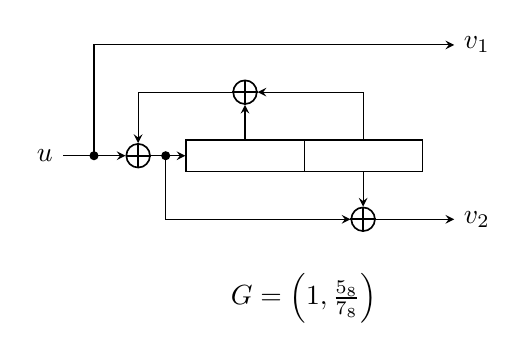
\begin{tikzpicture}[>=stealth]
\tikzstyle{rect} = [draw, rectangle, minimum width=30mm, inner sep=0mm, minimum height=4mm]
\tikzstyle{xor} = [draw, circle, semithick, minimum size=3mm, inner sep=0mm]

\node[rect] (rect) {};
\draw[-] (rect.north) -- (rect.south);

\node[xor] (rec) at ($(rect.west)+(-6mm,0)$) {};
\draw[semithick] (rec.north) -- (rec.south);
\draw[semithick] (rec.west) -- (rec.east);
\node[xor] (xor1) at ($(rect.north)+(-7.5mm,6mm)$) {};
\draw[semithick] (xor1.north) -- (xor1.south);
\draw[semithick] (xor1.west) -- (xor1.east);
\node[xor] (xor2) at ($(rect.south)+(7.5mm,-6mm)$) {};
\draw[semithick] (xor2.north) -- (xor2.south);
\draw[semithick] (xor2.west) -- (xor2.east);

\draw[<-] (rec.west) -- ++(-8mm,0) node [left] {$u$};
\draw[->] (rec.east) -- (rect.west);
\draw[->] ($(rect.north)+(-7.5mm,0)$) -- (xor1.south);
\draw[->] ($(rect.south)+(7.5mm,0)$) -- (xor2.north);
\draw[->] ($(rect.north)+(7.5mm,0)$) |- (xor1.east);
\draw[->] (xor1.west) -| (rec.north);

\draw[->] ($(rect.west)+(-2.5mm,0)$) |- (xor2.west);
\draw[->] (xor2.east) -- ($(rect.south east)+(4mm,-6mm)$) node [right] {$v_{2}$};
\draw[->] ($(rec.west)+(-4mm,0)$) |- ($(rect.north east)+(4mm,12mm)$) node [right] {$v_{1}$};

\draw[black, fill=black] ($(rect.west)+(-2.5mm,0)$) circle [radius=.5mm];
\draw[black, fill=black] ($(rec.west)+(-4mm,0)$) circle [radius=.5mm];

\node at ($(rect.south)+(0,-16mm)$) {$G=\left( 1,\frac{5_{8}}{7_{8}}\right)$};
\end{tikzpicture}
		}
		\caption{Rekursiv Systematischer Faltungskodierer}
		\label{abb:rsc_kodierer}
	\end{subfigure}
\caption{Verschiedene Faltungskodierertypen}
\label{abb:faltungskodierer_typen}
\end{figure}

\subsection{Systematische Faltungskodierer}
\label{kapitel:grundlagen_systematische_kodierer}
Bei systematischen Faltungskodierern entspricht ein Ausgang dem Eingangssignal. Die Quellinformation ist somit explizit im Kodewort enthalten. Abbildung \ref{abb:systematischer_kodierer} zeigt einen systematischen Faltungskodierer mit der Generatormatrix $G=\left( 4_{8},7_{8}\right)$. Systematische Faltungskodierer sind nie katastrophal, sind jedoch weniger robust wie nichtsystematische Faltungskodierer. \cite[S. 217]{schonfeld2012informations}

\subsection{Rekursiv systematische Faltungskodierer}
\label{kapitel:grundlagen_rsc}
Rekursiv systematische Faltungskodierer (RSC-Kodierer\footnote{Recursive Systematic Convolutional Coder}) weisen sowohl einen systematischen Ausgang als auch eine Rückkopplung des Schieberegisters zum Eingang vor. Aus Letzterem ergibt sich eine unendliche Einflusslänge. Das Eingangssignal ist wie bei allen systematischen Kodierern explizit im Kodewort enthalten. RSC-Kodierer sind aufgrund ihrer Verwendung in Turbo-Kodes von großer Bedeutung.
\\
Die Generatormatrix eines RSC-Kodierers mit einem Eingang wird folgendermaßen angegeben:
\begin{equation}
G=\left( 1, \frac{g_{1}}{g_{0}},\dots , \frac{g_{N-1}}{g_{0}} \right)
\end{equation}
Zumeist befindet sich an erster Stelle eine 1 und notiert den systematischen Ausgang. Das Polynom $g_{0}$ definiert die Rückkopplung des Kodierers. Die Polynome $g_{1}$ bis $g_{N-1}$ stellen die Polynome der nichtsystematischen Ausgänge dar \cite{morelos2006art}. Zur Definition eines RSC-Kodierers im späteren Programm müssen die oktalen Generatorpolynome der nichtsystematischen Ausgänge sowie der Rekursion angegeben werden. Das Polynom des systematischen Ausgangs muss nicht angegeben werden. Abbildung \ref{abb:rsc_kodierer} zeigt einen rekursiv systematischen Faltungskodierer für die Generatormatrix $G=\left( 1,\frac{5_{8}}{7_{8}}\right)$.

\subsection{Terminierung}
\label{kapitel:grundlageen_terminierung}
Die Terminierung bezeichnet nach der vollständigen Kodierung einer Nachricht das Zurückkehren des Kodierers in den Nullzustand. Dazu wird das Schieberegister mit $M$ 0-Bits befüllt. Die Terminierung wirkt sich positiv auf die Fehlerkorrekturfähigkeit bei der Dekodierung aus, da der Endzustand im Trellis bekannt ist. Jedoch geschieht dies auf Kosten der Koderate $R$, die durch die Terminierung sinkt. Die Koderate des terminierten Kodes $R_{t}$ berechnet sich für eine nicht terminierte Nachricht $\mathbf{u}=\left( u_{1},u_{2},\dots ,u_{k}\right)$ wie folgt:
\begin{equation}
R_{t}=\frac{k}{M+k}R
\end{equation}
Für lange Nachrichten ist $R_{t}\approx R$ und kann daher vernachlässigt werden.
\begin{figure}[t]
% trellis_terminiert.tex
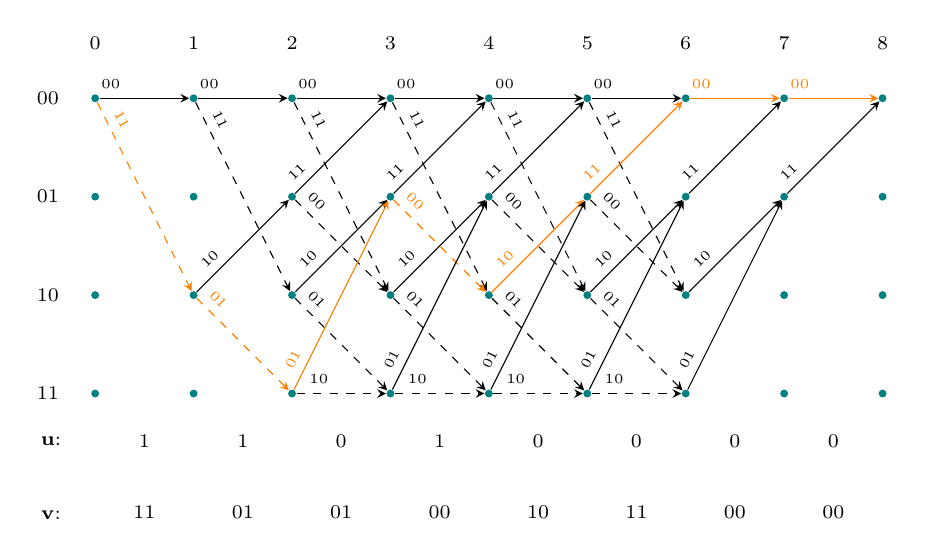
\begin{tikzpicture}[>=stealth, font=\scriptsize]
\tikzstyle{freestate} = [circle, teal, fill=teal, minimum size=1mm, inner sep=0mm]

\foreach \y in {0,...,3}
	\foreach \x in {0,...,8}
		\node[freestate] (node\y\x) at (1.25*\x,-1.25*\y) {};

\foreach \x in {0,...,8}
	\node (timelabel\x) [above of=node0\x, yshift=-3mm] {\x};
		
\node (statelabel0) [left of=node00, xshift=4mm] {00}; 
\node (statelabel1) [left of=node10, xshift=4mm] {01}; 
\node (statelabel2) [left of=node20, xshift=4mm] {10}; 
\node (statelabel3) [left of=node30, xshift=4mm] {11};

%t=0
\draw[->] (node00) -- (node01) node [sloped, above, very near start, font=\tiny] {00};
\draw[->, dashed, orange] (node00) -- (node21) node [sloped, above, very near start, font=\tiny] {11};

%t=1
\draw[->] (node01) -- (node02) node [sloped, above, very near start, font=\tiny] {00};
\draw[->, dashed] (node01) -- (node22) node [sloped, above, very near start, font=\tiny] {11};
\draw[->] (node21) -- (node12) node [sloped, above, near start, font=\tiny] {10};
\draw[->, dashed, orange] (node21) -- (node32) node [sloped, above, very near start, font=\tiny] {01};

%t=2
\draw[->] (node02) -- (node03) node [sloped, above, very near start, font=\tiny] {00};
\draw[->, dashed] (node02) -- (node23) node [sloped, above, very near start, font=\tiny] {11};
\draw[->] (node12) -- (node03) node [sloped, above, very near start, font=\tiny] {11};
\draw[->, dashed] (node12) -- (node23) node [sloped, above, very near start, font=\tiny] {00};
\draw[->] (node22) -- (node13) node [sloped, above, near start, font=\tiny] {10};
\draw[->, dashed] (node22) -- (node33) node [sloped, above, very near start, font=\tiny] {01};
\draw[->, orange] (node32) -- (node13) node [sloped, above, very near start, font=\tiny] {01};
\draw[->, dashed] (node32) -- (node33) node [sloped, above, near start, font=\tiny] {10};

%t=3
\draw[->] (node03) -- (node04) node [sloped, above, very near start, font=\tiny] {00};
\draw[->, dashed] (node03) -- (node24) node [sloped, above, very near start, font=\tiny] {11};
\draw[->] (node13) -- (node04) node [sloped, above, very near start, font=\tiny] {11};
\draw[->, dashed, orange] (node13) -- (node24) node [sloped, above, very near start, font=\tiny] {00};
\draw[->] (node23) -- (node14) node [sloped, above, near start, font=\tiny] {10};
\draw[->, dashed] (node23) -- (node34) node [sloped, above, very near start, font=\tiny] {01};
\draw[->] (node33) -- (node14) node [sloped, above, very near start, font=\tiny] {01};
\draw[->, dashed] (node33) -- (node34) node [sloped, above, near start, font=\tiny] {10};

%t=4
\draw[->] (node04) -- (node05) node [sloped, above, very near start, font=\tiny] {00};
\draw[->, dashed] (node04) -- (node25) node [sloped, above, very near start, font=\tiny] {11};
\draw[->] (node14) -- (node05) node [sloped, above, very near start, font=\tiny] {11};
\draw[->, dashed] (node14) -- (node25) node [sloped, above, very near start, font=\tiny] {00};
\draw[->,orange] (node24) -- (node15) node [sloped, above, near start, font=\tiny] {10};
\draw[->, dashed] (node24) -- (node35) node [sloped, above, very near start, font=\tiny] {01};
\draw[->] (node34) -- (node15) node [sloped, above, very near start, font=\tiny] {01};
\draw[->, dashed] (node34) -- (node35) node [sloped, above, near start, font=\tiny] {10};

%t=5
\draw[->] (node05) -- (node06) node [sloped, above, very near start, font=\tiny] {00};
\draw[->, dashed] (node05) -- (node26) node [sloped, above, very near start, font=\tiny] {11};
\draw[->,orange] (node15) -- (node06) node [sloped, above, very near start, font=\tiny] {11};
\draw[->, dashed] (node15) -- (node26) node [sloped, above, very near start, font=\tiny] {00};
\draw[->] (node25) -- (node16) node [sloped, above, near start, font=\tiny] {10};
\draw[->, dashed] (node25) -- (node36) node [sloped, above, very near start, font=\tiny] {01};
\draw[->] (node35) -- (node16) node [sloped, above, very near start, font=\tiny] {01};
\draw[->, dashed] (node35) -- (node36) node [sloped, above, near start, font=\tiny] {10};

%terminierung
%t=6
\draw[->, orange] (node06) -- (node07) node [sloped, above, very near start, font=\tiny] {00};
\draw[->] (node16) -- (node07) node [sloped, above, very near start, font=\tiny] {11};
\draw[->] (node26) -- (node17) node [sloped, above, near start, font=\tiny] {10};
\draw[->] (node36) -- (node17) node [sloped, above, very near start, font=\tiny] {01};
%t=7
\draw[->, orange] (node07) -- (node08) node [sloped, above, very near start, font=\tiny] {00};
\draw[->] (node17) -- (node08) node [sloped, above, very near start, font=\tiny] {11};

% input & output
\node (in0) at($(node30)!0.5!(node31)+(0,-.6)$) {1};
\node (in1) at($(node31)!0.5!(node32)+(0,-.6)$) {1};
\node (in2) at($(node32)!0.5!(node33)+(0,-.6)$) {0};
\node (in3) at($(node33)!0.5!(node34)+(0,-.6)$) {1};
\node (in4) at($(node34)!0.5!(node35)+(0,-.6)$) {0};
\node (in5) at($(node35)!0.5!(node36)+(0,-.6)$) {0};
\node (in6) at($(node36)!0.5!(node37)+(0,-.6)$) {0};
\node (in7) at($(node37)!0.5!(node38)+(0,-.6)$) {0};
\node (inlabel) at($(node30)+(-.56,-.6)$) {$\mathbf{u}$:};

\node (out0) [below=of in0, yshift=5mm] {11};
\node (out1) [below=of in1, yshift=5mm] {01};
\node (out2) [below=of in2, yshift=5mm] {01};
\node (out3) [below=of in3, yshift=5mm] {00};
\node (out4) [below=of in4, yshift=5mm] {10};
\node (out5) [below=of in5, yshift=5mm] {11};
\node (out6) [below=of in6, yshift=5mm] {00};
\node (out7) [below=of in7, yshift=5mm] {00};
\node (outlabel) at($(node30)+(-.56,-1.55)$) {$\mathbf{v}$:};

\end{tikzpicture}
\caption{Trellis für die terminierte Kodierung aus Beispiel~\ref{bsp:B5}.}
\label{abb:trellis_terminiert}
\end{figure}
\begin{beispiel}
Gegeben sei die Nachricht $\mathbf{u}=\left( 110100\right)$ aus Beispiel~\ref{bsp:B2}. Die Kodierung der terminierten Nachricht ist in Abbildung~\ref{abb:trellis_terminiert} zu sehen und ergibt das Kodewort $\mathbf{v}=\left( 11~01~01~00~10~11~00~00\right)$.
\label{bsp:B5}
\end{beispiel}

\subsection{Punktierung}
\label{kapitel:grundlagen_punktierung}
Zur Erhöhung der Koderate $R$ eines Kodes gibt es die Möglichkeit der Punktierung. Dabei werden bestimmte Bits vor der Übertragung anhand der sogenannten \emph{Punktierungsmatrix} $P \in {\left\lbrace 0,1 \right\rbrace}^{N\times \frac{p}{N}}$ gestrichen, wobei $p$ als Periode der Punktierungsmatrix bezeichnet wird und $P$ spaltenweise durchlaufen wird. Das Gewicht der Matrix $w(P)$ entspricht der Anzahl nicht punktierter Kodebits je Periode, d.h. der Anzahl an 1 in $P$.~\cite[S. 218]{schonfeld2012informations}
\\
\\
Die Koderate des punktierten Kodes $R_{p}$ berechnet sich wie folgt:
\begin{equation}
R_{p}=\frac{p}{w(P)}R
\end{equation}
Vor der Dekodierung erfolgt die Depunktierung, d.h. die punktierten Kodebits werden wieder eingefügt. Bei der soft decision Dekodierung wird der Signalwert 0, also genau zwischen den eigentlichen Signalwerten +1 und -1, an den zuvor punktierten Stellen eingefügt. Bei der hard decision Dekodierung wird das Bit 0 eingefügt.

\begin{beispiel}
Gegeben sei das Kodewort $\mathbf{v}=\left( 11~01~01~00~10~11\right)$ aus Beispiel~\ref{bsp:B2} und die Punktierungsmatrix
\begin{equation*}
P=
\begin{pmatrix}
1 & 0 & 1 \\
1 & 1 & 0 \\
\end{pmatrix}.
\end{equation*}
Nach der Punktierung ergibt sich das Kodewort $\mathbf{v_{p}}=\left( 11\ast 10\ast 00\ast 01\ast\right) = \left( 11100001\right)$. Die Koderate des punktierten Kodes beträgt $R_{p}=\frac{6}{4}\cdot\frac{1}{2}=\frac{3}{4}$.
\label{bsp:B6}
\end{beispiel}

\chapter{Verwendete Technologien}
\label{kapitel:technologien}
% technologien.tex
Dieses Kapitel über die verwendeten Technologien bei der Implementierung setzt sich folgendermaßen zusammen: Kapitel \ref{kapitel:R} behandelt die Programmiersprache R und die verwendete Entwicklungsumgebung RStudio. In Kapitel \ref{kapitel:rcpp} werden die Möglichkeiten der Einbindung von C/C++ Code, v.a. mithilfe des Pakets \emph{Rcpp}, beschrieben. Schließlich wird in Kapitel \ref{kapitel:rmarkdown} auf die Erstellung dynamischer Dokumente und Visualisierungen mittels \emph{RMarkdown}, \LaTeX\ und Ti\textit{k}Z.
\section{R, RStudio, Pakete}
\label{kapitel:R}
\begin{figure}[!t]
\centering
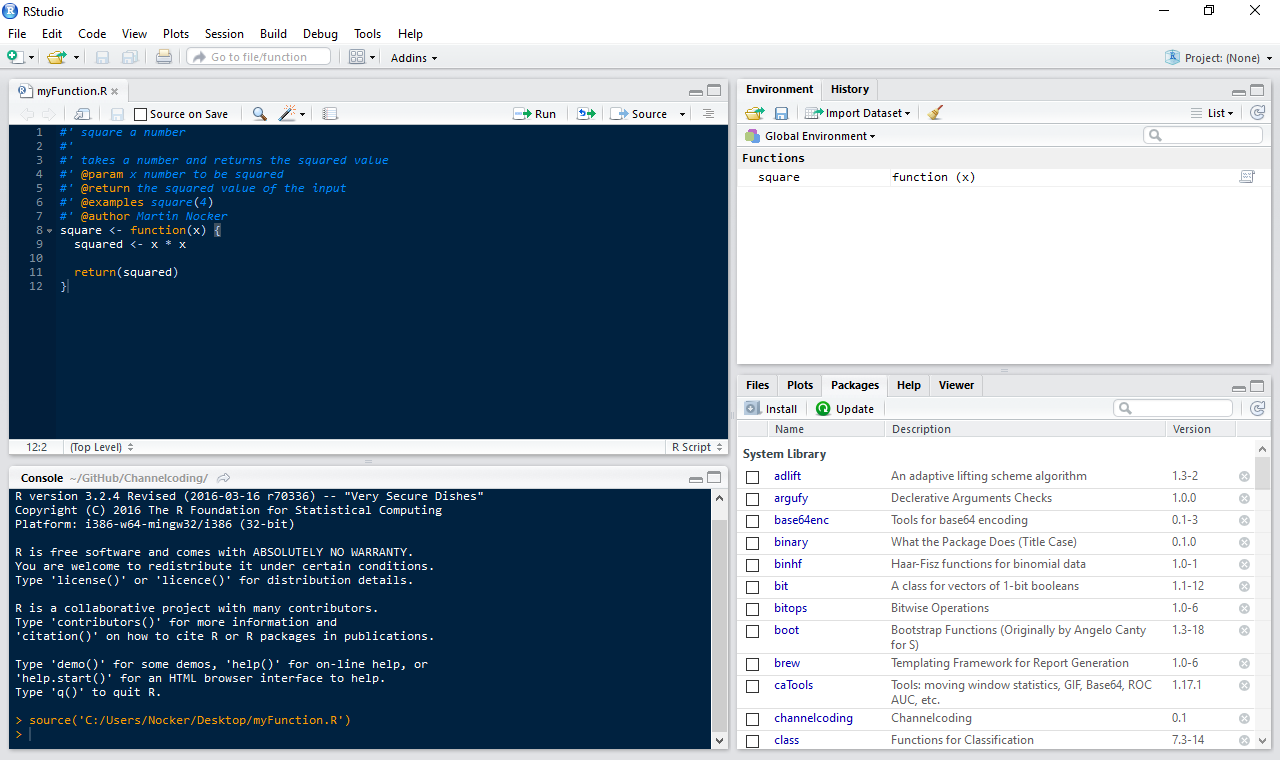
\includegraphics[width=\ScaleIfNeeded]{abbildungen/rstudio}
\caption{RStudio Standardansicht}
\label{abb:rstudio}
\end{figure}
% R
R ist eine, im Jahre 1992 entwickelte, schwach und dynamisch typisierte Programmiersprache, die vor allem in der Statistik für die Analyse von großen Datenmengen Anwendung findet. Ein weiteres Motiv für die Verwendung von R sind die vielseitigen Möglichkeiten, bei gleichzeitig einfacher Handhabung, graphischer Darstellungen großer Datenmengen. R-Code wird nicht kompiliert, sondern nur interpretiert und ist daher platformübergreifend verwendbar. Datentypen müssen zur Übersetzungszeit nicht bekannt sein. Die Typüberprüfung findet zur Laufzeit statt. Diese Eigenschaft erschwert das Finden von Fehlern im Code erheblich.
\\
\\
% R Pakete TODO! Cite
Der Funktionsumfang der Sprache kann durch sogenannte Pakete erweitert werden. Bei der Installation von R sind die wichtigsten Pakete inkludiert. Über Repositories wie CRAN\footnote{The Comprehensive R Archive Network: \url{https://cran.r-project.org/}} oder GitHub sind über 8000 zusätzliche Pakete (Stand: Mai 2016) für die verschiedensten Anwendungsbereiche verfügbar. Diese Vielfalt an Paketen ist ein Grund für den Erfolg von R [R Packages]. Pakete werden laufend aktualisiert und verbessert. Selbst entwickelte Pakete können via CRAN für andere Entwickler veröffentlicht werden, müssen jedoch strenge Auflagen zur Aufrechterhaltung der Konsistenz bei Inhalt, Form und Dokumentation der Pakete einhalten \cite{rmanual}.  
\\
\\
% Roxygen TODO! Lesen!
Ein wichtiges Paket welches im Rahmen dieser Arbeit verwendet wird ist \emph{roxygen}. Mithilfe dieses Pakets wird, ähnlich wie JavaDoc für Java, durch spezielle Kommentare und Annotations überhalb der Paketfunktionen automatisch die Paketdokumentation erstellt. Die roxygen-Kommentare der Paketfunktionen, die für wartbaren Code ohnehin unabdingbar sind, sind für den Entwickler erheblich angenehmer als die Paketdokumentation von Hand zu schreiben. Roxygen-Kommentare werden durch das Kommentarsymbol \# ' am Zeilenbeginn eingeleitet. Zu den wichtigsten Annotations gehören jene für die Beschreibung der Parameter (@param) und Rückgabewerte (@return) sowie Beispiele zur Ausführung der Funktion (@examples). Weiters wird über die @export Annotation geregelt welche Funktionen nach Auslieferung des Pakets von außen aufrufbar sind.
\\
\\
% RStudio
RStudio ist eine freie und open source Entwicklungsumgebung für R. RStudio verfügt über alle notwendigen Funktionalitäten für die Softwareentwicklung mit R und bietet darüber hinaus Funktionen für eine vereinfachte Entwicklung von R-Paketen an. Abbildung \ref{abb:rstudio} zeigt die Version 0.99.893. 
\section{C++, Rcpp}
\label{kapitel:rcpp}
Manchmal ist R-Code einfach nicht schnell genug. Typische Flaschenhälse sind Schleifen und rekursive Funktionen. Die Performance kann in solchen Fällen durch Auslagern von Funktionen und Algorithmen in C oder C++ erheblich verbessert werden, da der Code kompiliert und somit optimiert werden kann anstatt nur interpretiert zu werden.\\
R bietet drei Möglichkeiten C/C++ Code aufzurufen:
\begin{itemize}
	\item \emph{.C} native Schnittstelle
	\item \emph{.Call} Schnittstelle
	\item \emph{Rcpp} Paket
\end{itemize}
Die \emph{.C} Schnittstelle ist die einfachste Variante C Code auszuführen, jedoch auch jene mit den größten Einschränkungen. Im C Code sind keinerlei R Datentypen oder Funktionen bekannt. Alle Argumente sowie der Rückgabewert müssen als Zeiger in der Parameterliste übergeben werden deren Speicher vor dem Aufruf reserviert werden muss.
\\
\\
Bei der \emph{.Call} Schnittstelle handelt es sich um eine Erweiterung der \emph{.C} Schnittstelle. Die Implementierung ist komplexer, dafür sind R Datentypen verfügbar und es gibt die Möglichkeit eines Rückgabewerts mittels dem return Statements. \cite{wickham2015r}
\\
\\
Bei den ersten beiden Möglichkeiten muss der C Code vor dem Aufruf per Hand kompiliert und in der R Session geladen werden. Das \emph{Rcpp} Paket ermöglicht die Verwendung von C++ Code ohne diesen Aufwand. Im C++ Code stehen R Datentypen wie Vektoren, Matrizen oder Listen ohne kompliziertem Syntax zur Verfügung. Die Funktionsaufrufe sehen, im Gegensatz zu den ersten beiden Ausführungen, aus wie normale R Funktionsaufrufe und macht dadurch den Code erheblich lesbarer. Weiters stehen Vektorfunktionen zur Verfügung, d.h. eine auf einen Vektor angewandte Funktion wird auf jedes Vektorelement ausgeführt und erspart somit beispielsweise eine Schleife. Bei der Entwicklung eines eigenen Pakets ist es bei der Verwendung des \emph{Rcpp} Pakets zusammen mit RStudio sehr einfach C++ Code zu integrieren. Durch all diese Vorteile ist das \emph{Rcpp} Paket die zu wählende Schnittstelle. Während der Paketerzeugung kompiliert RStudio automatisch alle C++ Dateien und erstellt automatisch Wrapper-Funktionen, die den Zugriff auf die Funktionen erleichtern.
\\
\\
Die C++ Datei muss mit folgenden Zeilen starten:
\lstset{language=C++, numbers=none, basicstyle=\ttfamily}
\begin{lstlisting}
#include <Rcpp.h>
using namespace Rcpp;
\end{lstlisting}
Sowie jede Funktion, die in R verfügbar sein soll muss folgenden Präfix erhalten:
\begin{lstlisting}
// [[Rcpp::export]]
\end{lstlisting}
Die genaue Verwendung des \emph{Rcpp} Pakets ist in \cite{wickham2015advanced} beschrieben/ nachzulesen.
\section{RMarkdown, \LaTeX, Ti\textit{k}Z}
\label{kapitel:rmarkdown}
\begin{figure}[!t]
\centering

\includegraphics[width=\ScaleIfNeeded]{abbildungen/rmarkdown}
\caption{RMarkdown Überblick, Quelle: \cite{rmarkdown}}
\label{abb:rmarkdown}
\end{figure}
% R Markdown
Zur Erstellung von dynamischen Dokumenten wird das Paket \emph{RMarkdown} verwendet werden. Durch die Kombination der Syntax von Markdown, R, \LaTeX\ und HTML ergibt sich ein flexibles und einfaches Werkzeug. Die unterstützen Ausgabeformate beinhalten u.a. HTML, PDF, MS Word und Beamer (Präsentationen).
\\
\\
% R Markdown Workflow
Abbildung \ref{abb:rmarkdown} zeigt den Workflow für die Generierung eines dynamischen Dokuments mittels \emph{RMarkdown}. Der Markdown, R und \LaTeX\ Code wird zusammen mit dem gewünschten Ausgabeformat, wobei mehrere Angaben möglich sind, in die \emph{RMarkdown}-Datei (Dateiendung .rmd) geschrieben. Die RMD-Datei wird dem \emph{knitr} Paket übergeben, welches den R Code ausführt und eine neue Markdown-Datei (Dateiendung .md) erstellt, die den R Code und dessen Ergebnisse beinhaltet. Die erzeugte Markdown-Datei wird von \emph{pandoc} weiterverarbeitet, was für die Erstellung des endgültigen Dokuments im gewünschten Format zuständig ist. Bei der Verwendung von RStudio ist \emph{pandoc} automatisch verfügbar. Den eben beschriebenen Ablauf kapselt das \emph{RMarkdown}-Paket in einen einzigen \emph{render}-Funktionsaufruf.
\\
\\
% LaTeX, TikZ
Für die Erzeugung dynamischer Grafiken wird die Sprache Ti\textit{k}Z verwendet, die durch \LaTeX\ interpretiert wird. Mithilfe des Dokumenttyps Beamer in \LaTeX\ lassen sich Präsentationen erstellen. Die Grafiken und Inhalte können dadurch dynamisch ein- oder ausgeblendet werden oder farblich hervorgehoben werden. Dies ist insofern wertvoll, da Informationen, die Schritt für Schritt vervollständigt werden, es dem Benutzer leichter machen den Ablauf nachzuvollziehen. Damit zukünftige Studenten die Prinzipien von Faltungskodes besser verstehen werden die Visualisierungen der Kodierung und Dekodierung wie beschrieben sukzessive eingeblendet.

\chapter{Implementierung}
\label{kapitel:implementierung}
% implementierung.tex
Dieses Kapitel gibt einen Einblick in die Konzepte der Implementierung. Als Einstiegspunkt stand eine Referenzimplementierung\footnote{\url{http://vashe.org/turbo/turbo_example.c} (01.06.2016)} zur Verfügung, die den Dekodier-Algorithmus für Turbo-Kodes beinhaltet, jedoch für ein konkretes Beispiel. Dieser musste angepasst werden um für allgemeine Faltungskodes verwendbar zu sein.
\\
\\
Kapitel \ref{kapitel:implementierung_faltungskodierer} beinhaltet den Entwurf der Faltungskodierer-Datenstruktur. [TODO: Fertigstellung]
%Die Implementierung der Kodierung wird in Kapitel \ref{kapitel:implementierung_kodierung} beschrieben, die der Dekodierung in Kapitel \ref{kapitel:implementierung_dekodierung}.
%\\
%\\
%Aus Performancegründen Kodierung, Dekodierung in C++\\
%Weiters: Kodierer erzeugen, Depunktierung, Katastrophale Kodierer Prüfung (Polynom GGT mod 2)
%\\
%Parameterprüfung, Punktierung, ApplyNoise, Aufruf Visualisierung in R\\
%Referenzimplementierung
\section{Faltungskodierer}
\label{kapitel:implementierung_faltungskodierer}
Ein Faltungskodierer ist gegeben durch 
\begin{itemize}
\item $N$: Anzahl an Ausgangsbits je Eingangsbit,
\item $M$: Länge des Schieberegisters,
\item $G$: Vektor von Generatorpolynomen.
\end{itemize}
Die Angabe von $M$ ist hier redundant, jedoch Teil der Benutzereingabe zur Generierung eines Faltungskodierers, welche durch \cite{morelos2006art} inspiriert wurde.
\\
\\
Zur leichteren Implementierung der Kodierung und Dekodierung wird die Kodierer-Datenstruktur um folgende Elemente erweitert:
\begin{itemize}
\item eine \emph{Zustandsübergangsmatrix}, die angibt, in welchen Zustand der Kodierer bei einem Eingangsbit wechselt,
\item eine \emph{inverse Zustandsübergangsmatrix}, die angibt, aus welchem Zustand der Kodierer bei einem Eingangsbit kommt,
\item eine \emph{Ausgabematrix}, die angibt, welche Kodebits der Kodierer bei einem Eingangsbit in einem bestimmten Zustand ausgibt,
\item ein Flag zur Markierung rekursive systematischer Kodierer (RSC, siehe Kapitel~\ref{kapitel:grundlagen_rsc}),
\item ein \emph{Terminierungsvektor} die für rekursiver systematische Kodierer angibt, ob ein Eingangsbit 0 oder 1 in einem bestimmten Zustand für die Terminierung zu verwenden ist.
\end{itemize}
Die Implementierung der Matrizen wurde aus der Referenzimplementierung übernommen, musste jedoch erweitert werden, um für allgemeine Faltungskodes verwendbar zu sein. Für alle gilt, die Anzahl an Zeilen entspricht der Anzahl an Zuständen $2^{M}$. Der Zeilenindex entspricht dem Zustand. Die Zustandsübergangsmatrix sowie die Ausgabematrix besitzen jeweils zwei Spalten. Je eine Spalte steht für ein Eingangsbit (0 oder 1), wobei der Spaltenindex dem Eingangsbit entspricht. Die inverse Zustandsübergangsmatrix benötigt eine dritte Spalte. Für viele Kodierer (v.a. nicht-rekursive) tritt der Fall ein, dass nur durch \emph{ein bestimmtes} Eingangsbit in einen bestimmten Zustand gewechselt werden kann. Sei ein Zustand bspw. nur durch das Eingangsbit 0 erreichbar, so bedeutet das, dass es für diesen Zustand mit dem Bit 0 \emph{zwei} Vorgängerzustände gibt, für ein Eingangsbit 1 jedoch keinen Vorgänger. Diese zweite Möglichkeit wird in der dritten Spalte gespeichert.
\\
\\
Der Terminierungsvektor ist für nicht-rekursive Kodierer nicht notwendig, da ein Kode eines solchen Kodierers immer mit $M$ 0-Bits terminiert wird. Bei einem rekursiven Kodierer ist es nicht trivial zu sagen mit welchem Eingangsbit in einem bestimmten Zustand terminiert wird, um den Kodierer in den Nullzustand zu bringen. Dies hängt von der Definition des Rekursionpolynoms ab. Der Terminierungsvektor wird bei der Erzeugung rekursiver Kodierer berechnet.
\\
\\
Bei der Erzeugung von Faltungskodierern ist zu prüfen ob es sich um einen katastrophalen Kodierer handelt. RSC-Kodierer sind, wie in Kapitel \ref{kapitel:grundlagen_systematische_kodierer} beschrieben, nicht zu prüfen. Zur Prüfung wird nach dem Theorem von Massey-Sain (siehe Kapitel~\ref{kapitel:grundlagen_katastrophale_kodierer}) der größte gemeinsame Teiler der Generatorpolynome berechnet. Die Berechnung des größten gemeinsamen Teilers wurde mithilfe des euklidschen Algorithmus implementiert. Sowohl der euklidsche Algorithmus als auch die dafür notwendige binäre Polynomdivision wird an eine C++-Funktion delegiert.

\section{Kodierung}
\label{kapitel:implementierung_kodierung}
Bei Faltungskodes stellt die Kodierung den bei Weitem einfacheren Teil dar. Es muss lediglich jedes Bit der zu kodierenden Nachricht zusammen mit dem aktuellen Zustand, der nach jedem Bit mithilfe der Zustandsübergangsmatrix aktualisiert wird, auf die Ausgabematrix angewendet werden. Die Terminierung funktioniert analog, einzig das zu kodierende Bit muss ermittelt werden. Für RSC-Kodierer muss im Terminierungsvektor nachgeschaut werden, andernfalls ist das Terminierungsbit immer 0. Abgeschlossen wird die Kodierung mit dem Abbilden der Kodebits 0 bzw. 1 auf die Signalwerte +1 bzw. -1 nach Gleichung~\eqref{eq:bit_zu_signal_abbildung}. Algorithmus~\ref{algorithmus:kodierung} zeigt den Kodierungsalgorithmus.

\begin{algorithm}[H]
\renewcommand{\algorithmicforall}{\textbf{for each}}
\caption{Faltungskodierung}
\label{algorithmus:kodierung}
\begin{algorithmic}[1]
\STATE state $=0$, code $=$ result $=$ " "
\FORALL {bit \textbf{in} message}
   \STATE output $=$ output.matrix[state][bit]
	\STATE code $=$ $concat($code, output$)$
	\STATE state $=$ state.transition.matrix$[$state$][$bit$]$
\ENDFOR
\IF{terminate code}
   \FOR {$i=0$ \TO $M-1$}
      \STATE termination.bit $=$ rsc-coder $?$ termination.vector$[$state$]$ : $0$
      \STATE output $=$ output.matrix$[$state$][$termination.bit$]$
	   \STATE code $=$ $concat($code, output$)$
	   \STATE state $=$ state.transition.matrix$[$state$][$termination.bit$]$
   \ENDFOR
\ENDIF
\FORALL {bit \textbf{in} code}
   \STATE signal $=1-2$bit
   \STATE result $=$ $concat($result,signal$)$
\ENDFOR
\RETURN result
\end{algorithmic}
\end{algorithm}

\section{Dekodierung}
\label{kapitel:implementierung_dekodierung}
Die Dekodierung stellt den wesentlich komplexeren Teil der Faltungskodes dar. 

\begin{algorithm}[H]
\renewcommand{\algorithmicforall}{\textbf{for each}}
\caption{Faltungsdekodierung}
\label{algorithmus:dekodierung}
\begin{algorithmic}[1]
\STATE $NUM_STATES=2^{M}$
\FOR {$t=1$ \TO $length($message$)$}
   \FOR {$s=0$ \TO $NUM_STATES-1$}
   	\STATE $m_{1}=$ metric[t-1][prev.state1] + $\delta_{1}$
   	\STATE $m_{2}=$ metric[t-1][prev.state2] + $\delta_{2}$
      \STATE metric[t][s] = $min(m_{1},m_{2})$
      \STATE survivor.bit $=$ $xyz(0,1,min(min(m_{1},m_{2}))$
	\ENDFOR
\ENDFOR
\RETURN result
\end{algorithmic}
\end{algorithm}

\section{Rauschen}
\label{kapitel:implementierung_noise}
Um auch zeigen zu können, dass die Dekodierung auch tatsächlich für verrauschte Signale funktioniert, benötigt es eine Funktion, die die Übertragung einer Nachricht über einen verrauschten Kanal simuliert, d.h. das Signal mit Rauschen überlagert. Zum Signal soll ein additives weißes gaußsches Rauschen (AWGR oder AWGN\footnote{additive white Gaussian noise}) addiert werden um dieses zu verfälschen. [apply noise quelle] stellt eine alternative Implementierung zur eingebauten AWGN-Funktion in Matlab vor. Die Implementierung wurde übernommen bzw. nach R übersetzt. Durch die Möglichkeit das Signal-Rausch-Verhältnis über einen Parameter zu steuern, können verschiedene Übertragungskanäle simuliert und Nachrichten somit verschieden stark verrauscht werden. Der Benutzer kann dadurch herausfinden, ab wann eine Nachricht zu viel Rauschen enthält, um sie korrekt dekodieren zu können. Weiters kann nach mehrfacher Ausführung auf Fehlermuster geschlossen werden, mit denen die Dekodierung gut bzw. schlecht umgehen kann. Durch Versuche mit anderen Kanalkodierungs-Methoden können Vergleiche mit diesen angestellt werden. Die genannten Punkte helfen dem Benutzer sein Verständnis für Faltungskodes noch besser zu stärken.

\section{Punktierung}
\label{kapitel:implementierung_punktierung}
Punktierung leicht, jedoch Depunktierung vor der Dekodierung nicht trivial.

%\section{Visualisierung}
%\label{kapitel:implementierung_visualisierung}

\startlist[Funktionen]{lot}
\chapter{R-Paket Schnittstelle}
\label{kapitel:interface}
\definecolor{lightblue}{RGB}{150,180,255}
Dieses Kapitel soll als zusätzliche Hilfe (Nachschlagewerk) bei der Verwendung der R-Funktionen dienen, da hier die genauen Schnittstellen der Funktionen erklärt werden. Nachdem das Paket installiert ist, steht die Hilfe auch im RStudio zur Verfügung. Diese ist allerdings auf Englisch und nicht so umfangreich. Falls nach diesem Kapitel die Verwendung noch nicht komplett klar ist, kann man sich auch die Beispiele in Kapitel~\ref{cha:examples} anschauen. Für eine genaue Erklärung der Funktionen kann in Kapitel~\ref{cha:implementation} die genaue Implementierung nachgelesen werden und daraus auf die weitere Verwendung geschlossen werden.

In Kapitel~\ref{sec:interface_turboFunctions} sind alle Funktionen gelistet, die für das Kodieren und Dekodieren notwendig sind. Ein paar Hilfsfunktionen sind in Kapitel~\ref{sec:interface_helperFunctions} nachzuschlagen und die allgemeinen Funktionen, die für alle drei Verfahren notwendig sind, können im Kapitel~\ref{sec:interface_channelFunctions} nachgelesen werden. 
\newpage

\section{Turbo-Kode Funktionen}
\label{sec:interface_turboFunctions}

\subsection{Kodieren}
\label{sec:interface_encode}
\begin{longtable}{|p{\textwidth}|}
\hline
\rowcolor{lightblue}TurboEncode\\
\hline
\\
\texttt{TurboEncode(message, permutation.vector, coder.info, parity.index, punctuation.matrix, visualize)}\\
\\
Kodiert eine Nachricht mittels dem Turbo-Kode-Verfahren. Dabei wird die Nachricht in zwei systematische Kodierer geschickt und am Ausgang wird das Ergebnis der beiden Kodierer mit der Originalnachricht zusammengesetzt. Falls eine Punktierungsmatrix mitgegeben wird, erfolgt am Ende die Punktierung und somit die Erhöhung der Koderate.\\
\\
\textbf{Argumente:}\\
\texttt{message} - Nachricht die kodiert wird. (0er und 1er)\\
\texttt{permutation.vector} - Permutationsvektor der für den Interleaver verwendet wird. Standard: \texttt{PRIMITIVE (root=0)}\\
\texttt{coder.info} - Faltungskodierer der mit den Funktionen \texttt{ConvGenerateEncoder, ConvGenerateRscEncoder} erzeugt werden kann. Muss ein systematischer Kodierer sein, also ein RSC oder Ausgang 1 muss durchgeschalten sein. Standard: \texttt{ConvGenerateRscEncoder(2,2,c(5,7))}\\
\texttt{parity.index} - Gibt an welcher Ausgang vom mitgegebenen Kodierer verwendet wird. Standard: letzter Ausgang\\
\texttt{punctuation.matrix} - Die Matrix wird am Ende des Kodiervorgangs zur Punktierung verwendet. Standard: keine Punktierung\\
\texttt{visualize} - Wenn \texttt{TRUE} wird PDF-Bericht erstellt. Standard: \texttt{FALSE}\\
\\
\textbf{Rückgabewert:}\\
Die kodierte Nachricht mit den Signalwerten -1 und 1, welche die Bits 1 und 0 darstellen. Falls punktiert wurde, wird eine Liste mit dem Originalkode und dem punktierten Kode zurückgegeben.\\
\\
\hline
\caption[TurboEncode]{TurboEncode - Funktionserklärung}
\end{longtable}

\subsection{Dekodieren}
\label{sec:interface_decode}
\begin{longtable}{|p{\textwidth}|}
\hline
\rowcolor{lightblue}TurboDecode\\
\hline
\\
\texttt{TurboDecode(code, permutation.vector, iterations, coder.info, parity.index, punctuation.matrix, visualize)}\\
\\
Dekodiert eine Nachricht mittels dem Turbo-Kode-Verfahren. Dabei werden zuerst die Punktierungsbits wieder eingefügt, falls Punktierung verwendet wurde. Danach erfolgt die Dekodierung, wobei die Ergebnisse der Dekodierer als Eingang des Nächsten verwendet werden. Dieser Vorgang wird mehrmals iterativ ausgeführt, je nach Anzahl der gewählten Iterationen.\\
\\
\textbf{Argumente:}\\
\texttt{code} - Nachricht die dekodiert wird. Der genaue Signalpegel wird verwendet.\\
\texttt{permutation.vector} - Permutationsvektor der für den Interleaver verwendet wird. Standard: \texttt{PRIMITIVE (root=0)}\\
\texttt{iterations} - Anzahl der Dekodierungsiterationen. Standard: 1\\
\texttt{coder.info} - Faltungskodierer der bei der Kodierung bereits verwendet wurde. Standard: \texttt{ConvGenerateRscEncoder(2,2,c(5,7))}\\
\texttt{parity.index} - Gibt an welcher Ausgang vom mitgegebenen Kodierer verwendet wird. Standard: letzter Ausgang\\
\texttt{punctuation.matrix} - Die mitgegebene Punktierungsmatrix wird am Anfang des Dekodiervorgangs,  für das Einfügen der jeweiligen Bits verwendet. Standard: keine Punktierung\\
\texttt{visualize} - Wenn \texttt{TRUE} wird PDF-Bericht erstellt. Standard: \texttt{FALSE}\\
\\
\textbf{Rückgabewert:}\\
Liste welche die dekodierte Nachricht und die genau berechneten Soft-Werte enthält.\\
\\
\hline
\caption[TurboDecode]{TurboDecode - Funktionserklärung}
\end{longtable}
\newpage

\subsection{Simulation von Turbo-Kodes}
\label{sec:interface_simulation}
\begin{longtable}{|p{\textwidth}|}
\hline
\rowcolor{lightblue}TurboSimulation\\
\hline
\\
\texttt{TurboSimulation(coder, permutation.type, permutation.args, decode.iterations, msg.length, min.db, max.db, db.interval, iterations.per.db, punctuation.matrix, visualize)}\\
\\
Automatische Simulation eines Kodierungs- und Dekodierungsverfahrens von Turbo-Kodes. Nach dem Kodieren wird der resultierende Kode verrauscht und im Anschluss dekodiert. Für das jeweilige Signal/Rausch-Verhältnis wird dieses Verfahren mehrmals (\texttt{iterations.per.db}) wiederholt und am Ende ein Durchschnitt der Bitfehlerrate berechnet.\\
\\
\textbf{Argumente:}\\
\texttt{coder} - Kodierer der für Kodierung und Dekodierung verwendet wird. Kann mittels den Funktionen \texttt{ConvGenerateEncoder, ConvGenerateRscEncoder} erzeugt werden. Standard: \texttt{ConvGenerateRscEncoder(2,2,c(5,7))}\\
\texttt{permutation.type} - Typ des Permutationsvektors. Standard: \texttt{PRIMITIVE}\\
\texttt{permutation.args} - Argumente für die Erzeugung des Permutationsvektors. Standard: \texttt{list(root=0)}\\
\texttt{decode.iterations} - Anzahl von Iterationen bei der Dekodierung. Standard: 5\\
\texttt{msg.length} - Länge der Nachricht. Standard: 100\\
\texttt{min.db} - Untergrenze des Signal/Rausch-Verhältnisses. Standard: 0.1\\
\texttt{max.db} - Obergrenze des Signal/Rausch-Verhältnisses. Standard: 2.0\\
\texttt{db.interval} - Schrittweite pro Erhöhung des Signal/Rausch-Verhältnisses. Standard: 0.1\\
\texttt{iterations.per.db} - Iterationen pro Signal/Rausch-Verhältnis zur Durchschnittsbildung. Standard: 100\\
\texttt{punctuation.matrix} - Verwendete Punktierungsmatrix. Standard: wird nicht punktiert\\
\texttt{visualize} - Wenn \texttt{TRUE} wird PDF-Bericht erstellt. Standard: \texttt{FALSE}\\
\\
\textbf{Rückgabewert:}\\
Dataframe das für jedes Signal/Rausch-Verhältnis eine Bitfehlerrate beinhaltet.\\
\\
\hline
\caption[TurboSimulation]{TurboSimulation - Funktionserklärung}
\end{longtable}

\section{Hilfsfunktionen}
\label{sec:interface_helperFunctions}

\subsection{Permutationsvektor erzeugen}
\label{sec:interface_permutation}
\begin{longtable}{|p{\textwidth}|}
\hline
\rowcolor{lightblue}TurboGetPermutation\\
\hline
\\
\texttt{TurboGetPermutation(message.length, coder.info, type, args, visualize)}\\
\\
Erzeugt einen Permutationsvektor für die Interleaver beim Turbo-Kode-Verfahren. Dabei können verschiedene Typen von Permutationen ausgewählt werden (RANDOM, PRIMITIVE, CYCLIC, BLOCK, HELICAL, DIAGONAL). Die genauere Erklärung des jeweiligen Typs findet sich im Kapitel \ref{cha:implementation}. Den jeweiligen Typen müssen spezielle Argumente in einer Liste mitgegebenen werden:
\begin{itemize}
\item RANDOM: Benötigt keine Argumente, wird komplett zufällig erstellt.
\item PRIMITVE: Erzeugt einen Vektor (1,2,3...) und schiebt diesen um den \emph{root}-Wert.
\item CYCLIC: Benötigt die Argumente \emph{cols} und \emph{rows} für die Erzeugung der Matrix und \emph{distance} um den Permutationsvektor zu erzeugen.
\item BLOCK: Benötigt die Argumente \emph{cols} und \emph{rows} für die Erzeugung der Matrix. Matrix wird von links nach rechts befüllt und von oben nach unten ausgelesen.
\item HELICAL: Benötigt die Argumente \emph{cols} und \emph{rows} für die Erzeugung der Matrix. Matrix wird von links nach rechts befüllt und von links oben nach rechts unten ausgelesen.
\item DIAGONAL: Benötigt die Argumente \emph{cols} und \emph{rows} für die Erzeugung der Matrix. Matrix wird von links nach rechts befüllt und dann diagonal ausgelesen.
\end{itemize} \\
\\
\textbf{Argumente:}\\
\texttt{message.length} - Länge der Nachricht die kodiert werden möchte.\\
\texttt{coder.info} - Faltungskodierer der mit den Funktionen \emph{ConvGenerateEncoder, ConvGenerateRscEncoder} erzeugt werden kann. Standard: \emph{ConvGenerateRscEncoder(2,2,c(5,7))}\\
\texttt{type} - Typ des erzeugten Permutationsvektors. Standard: RANDOM\\
\texttt{args} - Argumente für den jeweiligen Typ in einer Liste. Standard: NULL\\
\texttt{visualize} - Wenn TRUE wird die Permutationsmatrix dargestellt. Standard: FALSE\\
\\
\textbf{Rückgabewert:}\\
Permutationsvektor mit der richtigen Länge für die mitgegebene Nachricht und Kodierer.\\
\\
\hline
\caption{TurboGetPermutation - Funktionserklärung}
\end{longtable}

\subsection{Punktierungsmatrix erzeugen}
\label{sec:interface_punctuation}
\begin{longtable}{|p{\textwidth}|}
\hline
\rowcolor{lightblue}TurboGetPunctuationMatrix\\
\hline
\\
\texttt{TurboGetPunctuationMatrix(punctuation.vector, visualize)}\\
\\
Erzeugt eine Punktierungsmatrix von einem mitgegebenen Vektor für das Turbo-Kode-Verfahren (drei Zeilen). Es dürfen keine Null-Spalten entstehen!\\
\\
\textbf{Argumente:}\\
\texttt{punctuation.vector} - Vektor der in eine Punktierumatrix transformiert wird. Eine 1 behaltet das Bit, eine 0 verwirft das Bit.\\
\texttt{visualize} - Wenn \texttt{TRUE} wird Punktierungsmatrix dargestellt. Standard: \texttt{FALSE}\\
\\
\textbf{Rückgabewert:}\\
Punktierungsmatrix die für das Turbo-Kode-Verfahren geeignet ist.\\
\\
\hline
\caption[TurboGetPunctuationMatrix]{TurboGetPunctuationMatrix - Funktionserklärung}
\end{longtable}
\newpage

\subsection{Öffnen der erzeugten Visualisierungen}
\label{sec:interface_openPDF}
\begin{longtable}{|p{\textwidth}|}
\hline
\rowcolor{lightblue}TurboOpenPDF\\
\hline
\\
\texttt{TurboOpenPDF(encode, punctured, simulation)}\\
\\
Öffnet die mit \emph{TurboEncode, TurboDecode, TurboSimulation} bereits erzeugten PDF-Berichte. Die Dateien liegen im Paket-Ordner im Installationsverzeichnis von R.\\
\\
\textbf{Argumente:}\\
\texttt{encode} - Wenn TRUE werden PDFs vom Kodierungs-, bei FALSE vom Dekodierungsverfahren geöffnet. Standard: TRUE\\
\texttt{punctured} - Wenn TRUE werden PDFs mit Punktierungsverfahren geöffnet. Standard: FALSE\\
\texttt{simulation} - Wenn TRUE öffnet sich der Bericht der Simulation. Standard: FALSE\\
\\
\hline
\caption{TurboOpenPDF - Funktionserklärung}
\end{longtable}
\newpage

\section{Kanalkodierungsfunktionen im Paket}
\label{sec:interface_channelFunctions}

\subsection{Rauschen hinzufügen}
\label{sec:interface_applyNoise}
\begin{longtable}{|p{\textwidth}|}
\hline
\rowcolor{lightblue}
ApplyNoise\\
\hline
\\
\texttt{ApplyNoise(msg, SNR.db, binary)}\\
\\
Verrauscht ein Signal basierend auf das AWGN (additive white gaussian noise) Modell. Das ist das Standardmodell für die Simulation eines Übertragungskanals.\\
\\
\textbf{Argumente:}\\
\texttt{msg} - Nachricht die verrauscht wird.\\
\texttt{SNR.db} - Signal/Rausch-Verhältnis des Übertragungskanals. Standard: 3.0\\
\texttt{binary} - Blockkode-Parameter. Nicht zu verwenden! Standard: FALSE\\
\\
\textbf{Rückgabewert:}\\
Verrauschtes Signal.\\
\\
\hline
\caption{ApplyNoise - Funktionserklärung}
\label{func:applynoise}
\end{longtable}

\subsection{Simulation von Block-, Faltungs- und Turbo-Kodes}
\label{sec:interface_channelcodingSimulation}
% ChannelcodingSimulation.tex
\begin{longtable}{|p{\textwidth}|}
\hline
\rowcolor{lightblue}ChannelcodingSimulation\\
\hline
\\
\texttt{ChannelcodingSimulation(msg.length, min.db, max.db, db.interval, iterations.per.db, turbo.decode.iterations, visualize)}\\
\\
Simulation of channelcoding techniques (blockcodes, convolutional codes and turbo codes) and comparison of their bit-error-rates.\\
\\
\textbf{Arguments:}\\
\texttt{msg.length} - Message length of the randomly created messages to be encoded. Default: 100\\
\texttt{min.db} - Minimum SNR to be tested. Default: 0.1\\
\texttt{max.db} - Maximum SNR to be tested. Default: 2.0\\
\texttt{db.interval} - Step between two SNRs tested. Default: 0.1\\
\texttt{iterations.per.db} - Number of encode and decode processes per SNR. Default: 100\\
\texttt{turbo.decode.iterations} - Number of decoding iterations inside the turbo decoder. Default: 5\\
\texttt{visualize} - If true a PDF report is generated. Default: FALSE\\
\\
\textbf{Returns:}\\
Distorted message containing noise.\\
\\
\hline
\end{longtable}

\subsection{Darstellung verschiedener Simulationen}
\label{sec:interface_plotSimulationData}
% PlotSimulationData.tex
\begin{longtable}{|p{\textwidth}|}
\hline
\rowcolor{lightblue}PlotSimulationData\\
\hline
\\
\texttt{PlotSimulationData(\dots)}\\
\\
Stellt mehrere mitgegebene Dataframes in einem Diagramm dar. Damit kann man verschiedene Kanalkodierungsverfahren miteinander vergleichen.\\
\\
\textbf{Argumente:}\\
\texttt{\dots} - Dataframes die mit den Simulationsfunktionen erzeugt wurden.\\	
\\
\hline
\caption[PlotSimulationData]{PlotSimulationData - Funktionserklärung}
\end{longtable}
\stoplist[Funktionen]{lot}

\chapter{Visualisierung}
\label{kapitel:visualisierung}
% visualisierung.tex
Wird der \texttt{visualize}-Parameter bei der Ausführung einer R-Paket-Funktion auf \texttt{TRUE} gesetzt, wird ein \texttt{RMarkdown}-Skript ausgeführt. Dieses generiert eine  Präsentation vom \LaTeX -Dokumenttyp \emph{Beamer} mit Informationen und Visualisierungen zur ausgeführten Funktion.
\\
Die erzeugten Präsentationen liegen innerhalb des Programmverzeichnisses von R im Installationsordner des Pakets. Dort gibt es den Ordner \emph{pdf}, in dem sich die Dokumente befinden. Möchte man die Dokumente von RStudio aus öffnen, anstatt die Dokumente in der Verzeichnisstruktur suchen zu müssen, kann die \texttt{ConvOpenPDF}-Funktion (siehe Funktion~\ref{funktion:ConvOpenPDF}) verwendet werden. Möchte man die Dokumente zu einem späteren Zeitpunkt erneut einsehen, wird empfohlen eine Kopie der Datei abzuspeichern, da bei einer erneuten Ausführung der gleichen Funktion inklusive Visualisierung das zuvor erzeugte Dokument im \emph{pdf}-Ordner überschrieben wird. Die vom \texttt{RMarkdown}-Skript erzeugten \LaTeX -Dateien, aus denen die Beamer Präsentationen generiert werden, liegen ebenfalls im selben Verzeichnis.
\\
Da einerseits der Platz auf einer Folie begrenzt ist und andererseits Visualisierungen zu Lehrzwecken nur für kurze Bitsequenzen sinnvoll sind, gibt es Einschränkungen für die in einer Visualisierung verwendeten Nachrichten und Kodierer. Eine Visualisierung der Kodierung bzw. Dekodierung erfolgt für Nachrichten bzw. dekodierte Nachrichten inklusive Terminierungsbits bei einer Länge von bis zu 14 Bits. Bei einem Faltungskodierer mit einer Schieberegisterlänge von vier oder größer erfolgt keine Visualisierung der Dekodierung, da das Trellis zu groß ist. Bei der Kodierung wird nur das Zustandsdiagramm nicht abgebildet.
\\
Bei den folgenden Beispielen der Visualisierungen wurde stets punktiert, da ohne Punktierung die Informationen zur Punktierung in den Präsentationen fehlen und somit auch nicht erläutert werden können.
\\
\\
Der weitere Kapitelinhalt setzt sich folgendermaßen zusammen: Die Kapitel~\ref{kapitel:visualisierung_kodierung} bzw. \ref{kapitel:visualisierung_dekodierung} beinhalten Erläuterungen zur Visualisierung der Kodierung bzw. Dekodierung. Kapitel~\ref{kapitel:visualisierung_simulation} beschreibt die Visualisierung der Simulation.
\section{Kodierung}
\label{kapitel:visualisierung_kodierung}
% allg. Informationen
Bei der Kodierung befinden sich auf den ersten Folien allgemeine Informationen zum verwendeten Faltungskodierer. Abbildung~\ref{abb:folie_kodierer_kennwerte} zeigt die Folie mit den Kennwerten des Faltungskodierers: Anzahl an Ausgängen $N$, Länge des Schieberegisters $M$, Generatorpolynome, Punktierungsmatrix und Koderate. Auf den nächsten beiden Folien werden die Zustandsübergangsmatrix und die Ausgabematrix abgebildet. In Abbildung~\ref{abb:folie_zustandsübergangsmatrix} ist die Folie der Zustandsübergangsmatrix zu sehen. Analog dazu wird die Ausgabematrix auf der nächsten Folie veranschaulicht. Diese wird aus Platzgründen hier nicht abgebildet.
\begin{figure}[th]
	\centering
	\begin{subfigure}{0.48\textwidth}
		\centering
		\fbox{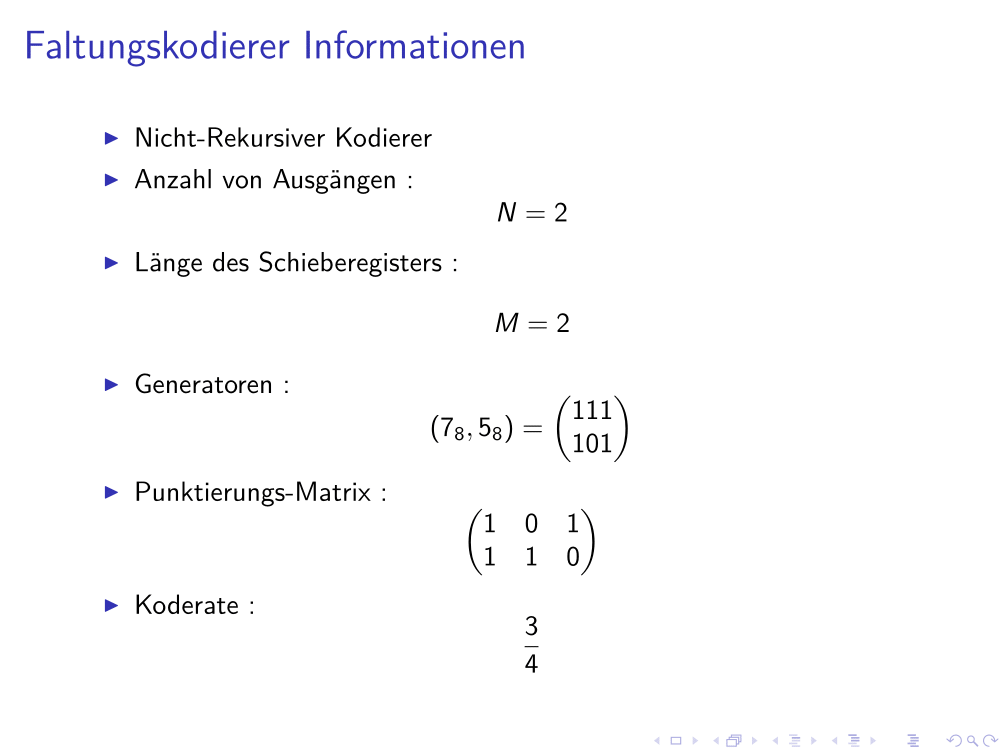
\includegraphics[width=0.99\textwidth]{abbildungen/folie_kodierung_info}}
		\caption{Folie mit Kodierer-Kennwerten}
		\label{abb:folie_kodierer_kennwerte}
	\end{subfigure}
	\quad % spacing between subfigures
	\begin{subfigure}{0.48\textwidth}
		\centering
		\fbox{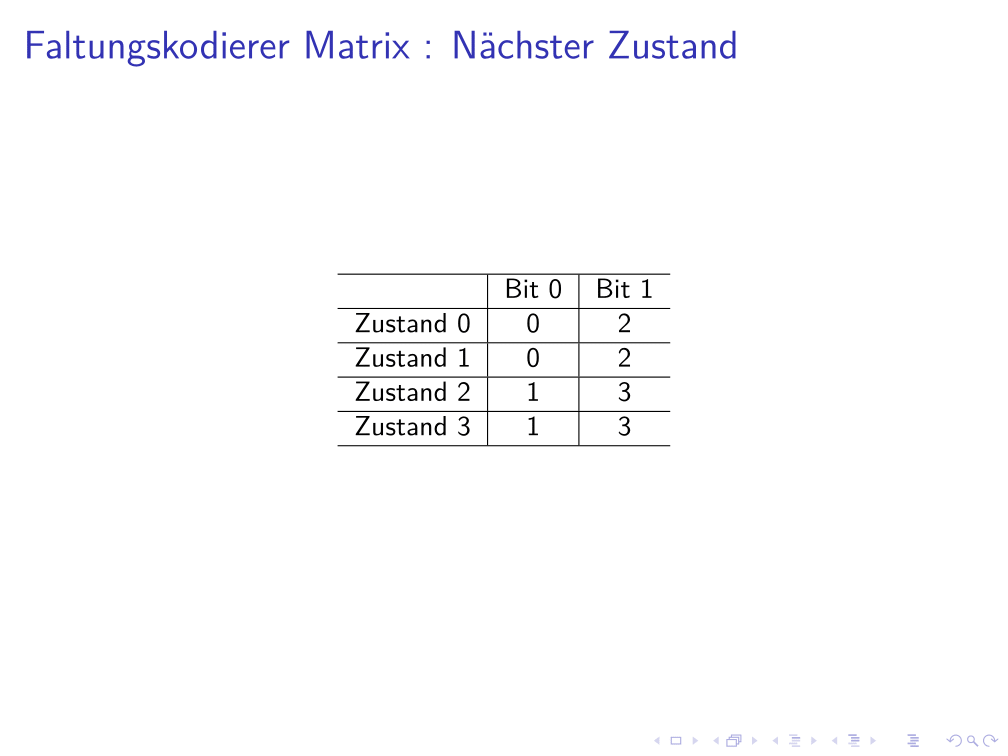
\includegraphics[width=0.99\textwidth]{abbildungen/folie_kodierung_matrix_zustand}}
		\caption{Folie mit Zustandsübergangsmatrix}
		\label{abb:folie_zustandsübergangsmatrix}
	\end{subfigure}
	\caption{Folien mit allgemeinen Informationen zum Faltungskodierer}
	\label{abb:folie_allg_info_kodierer}
\end{figure}
% Kodierung
Anschließend folgt die Visualisierung der Kodierung. Dabei wird die zu kodierende Nachricht Bit für Bit auf einer eigenen Folie verarbeitet. Abbildung~\ref{abb:folie_kodierung} zeigt die ersten beiden Schritte sowie den letzten Schritt der Kodierung. In Abbildung~\ref{abb:folie_kodierung_1} ist die Folie vor der Kodierung des ersten Bits zu sehen. Zunächst ist die zu kodierende Nachricht (Input), das Zustandsübergangsdiagramm, sowie eine noch nicht befüllte Kodierungstabelle zu sehen. Das Kodewort wird auf den folgenden Folien Schritt für Schritt erarbeitet. Durch diese Herangehensweise ist die Kodierung für den Benutzer einfach nachzuvollziehen. Abbildung~\ref{abb:folie_kodierung_2} zeigt die Folie der Kodierung des ersten Bits. Das erste Bit des Inputs, der aktuelle Zustand, der Folgezustand sowie der resultierende Output werden in eine neue Zeile der Kodierungstabelle geschrieben. Der aktuelle Zustand sowie der entsprechende Übergang werden im Diagramm farblich hervorgehoben, um die Kodierung auch im Zustandsdiagramm verfolgen zu können. Der Output wird auch unterhalb der Tabelle eingetragen und wächst mit jedem Schritt bis schlussendlich die gesamte Nachricht kodiert wurde. Die Visualisierung am Ende der Kodierung ist in Abbildung~\ref{abb:folie_kodierung_3} zu sehen. Die Bits unterhalb der horizontalen Trennlinie in der Tabelle stellen die Terminierungsbits dar.
\begin{figure}[th]
	\centering
	\begin{subfigure}{0.48\textwidth}
		\centering
		\fbox{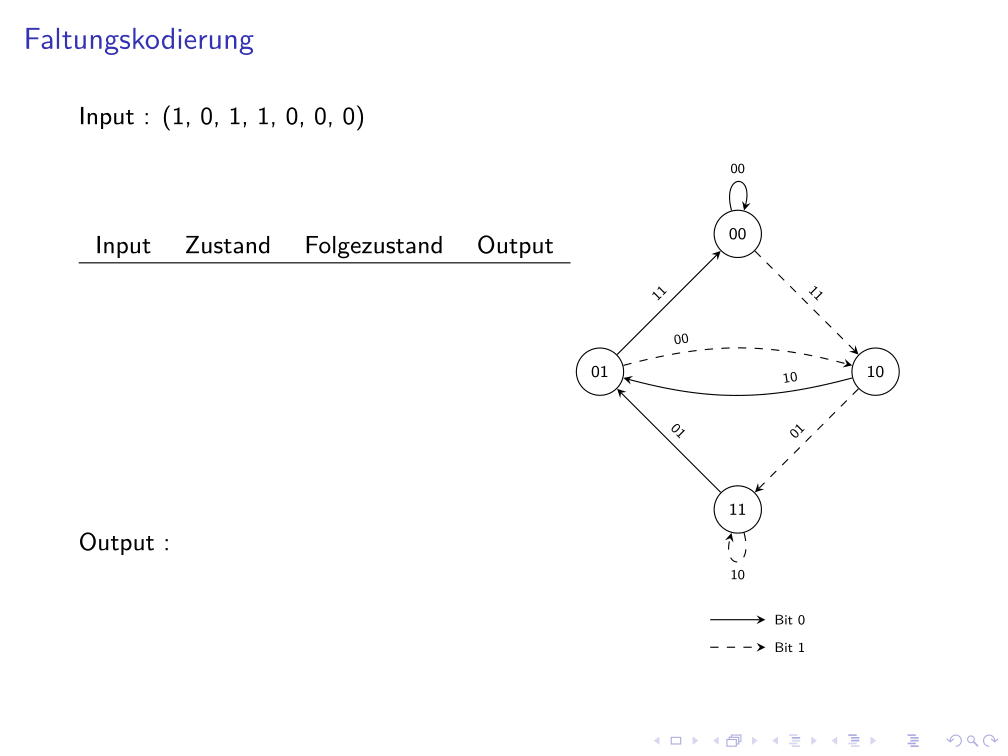
\includegraphics[width=0.99\textwidth]{abbildungen/folie_kodierung_1}}
		\caption{}
		\label{abb:folie_kodierung_1}
	\end{subfigure}
	\quad
	\begin{subfigure}{0.48\textwidth}
		\centering
		\fbox{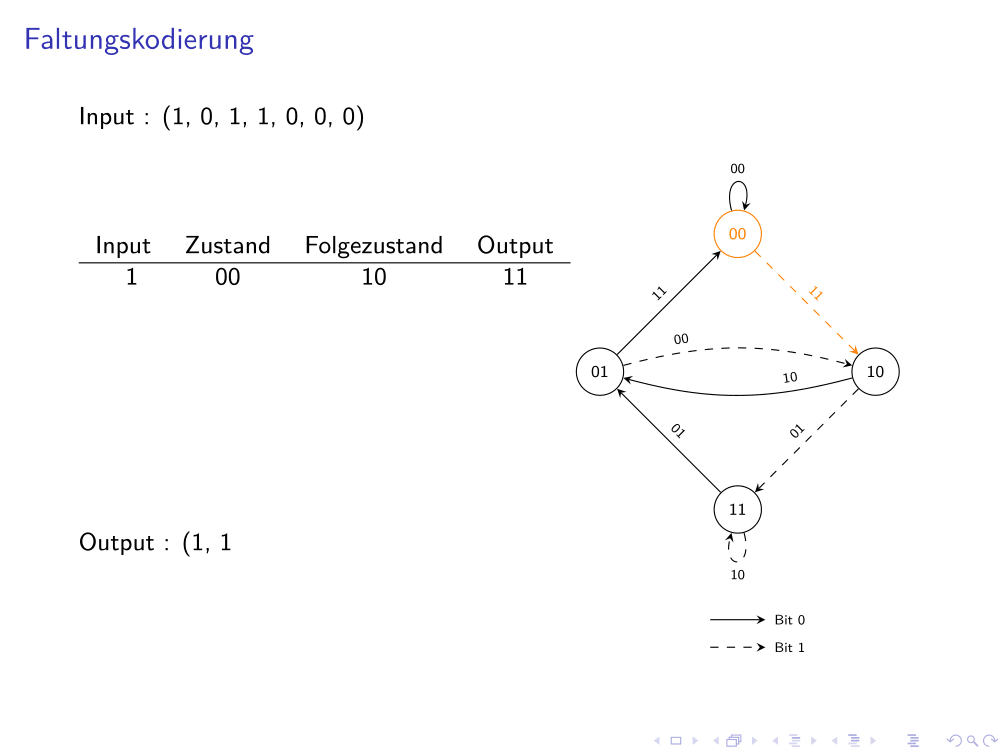
\includegraphics[width=0.99\textwidth]{abbildungen/folie_kodierung_2}}
		\caption{}
		\label{abb:folie_kodierung_2}
	\end{subfigure}
	\par\bigskip
	\begin{subfigure}{0.7\textwidth}
		\centering
		\fbox{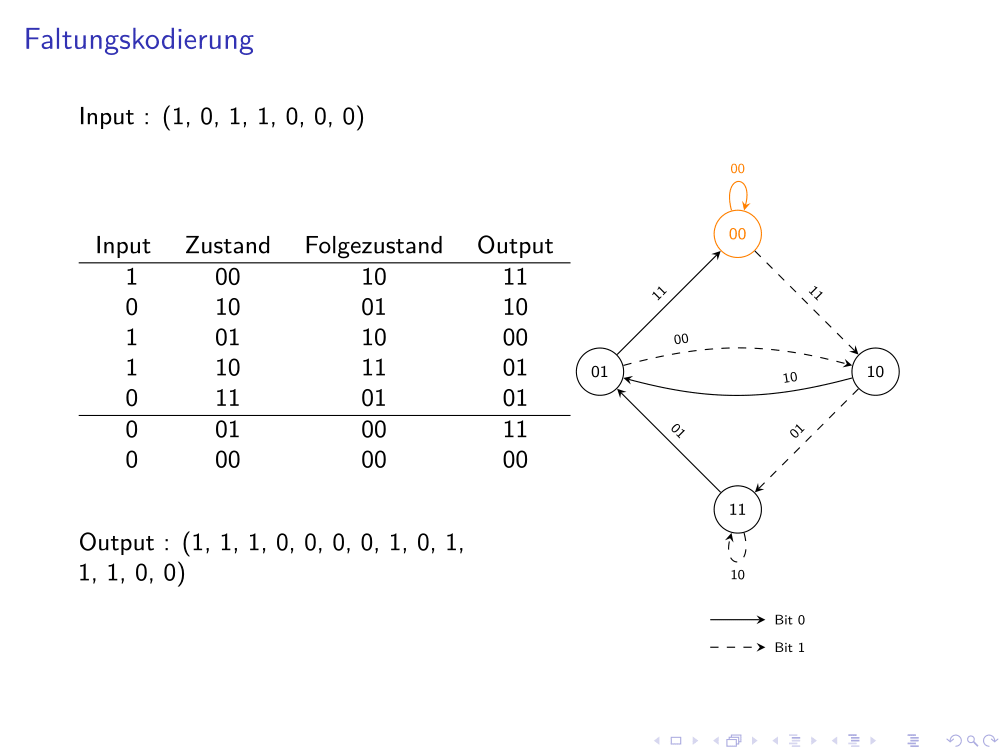
\includegraphics[width=0.99\textwidth]{abbildungen/folie_kodierung_3}}
		\caption{}
		\label{abb:folie_kodierung_3}
	\end{subfigure}
	\caption{Folien der Kodierung}
	\label{abb:folie_kodierung}
\end{figure}
% Kode zu Signal
Da die Kodierungsfunktion nicht die Bitwerte des Kodeworts zurückliefert, sondern die Signalwerte (für eine Übertragung über einen Kanal) wird auf einer weiteren Folie, wie in Abbildung~\ref{abb:folie_bit_zu_signal_abbildung} zu sehen, die Abbildung der Kodebits zu den Signalpegeln nach Gleichung~\eqref{eq:bit_zu_signal_abbildung} dargestellt.
\begin{figure}[th]
	\centering
	\fbox{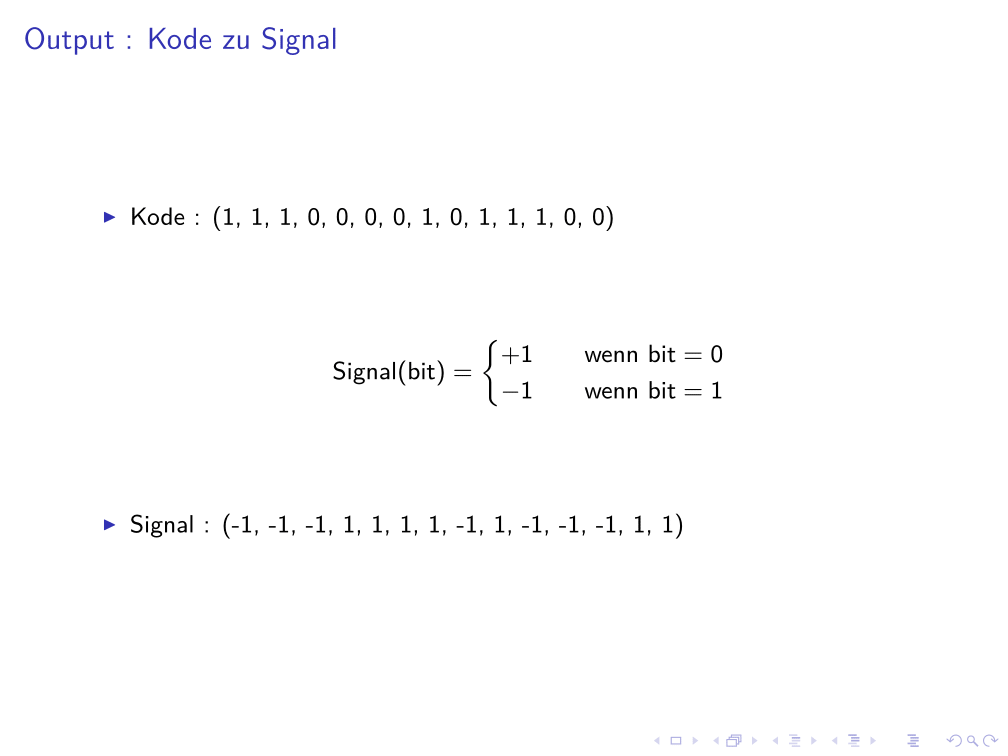
\includegraphics[width=0.7\textwidth]{abbildungen/folie_kodierung_bit_zu_signal}}
	\caption{Folie mit der Abbildung der Kodebits zu den Signalpegeln}
	\label{abb:folie_bit_zu_signal_abbildung}
\end{figure}
% Punktierung
Abbildung~\ref{abb:folie_punktierung} zeigt die Folie der Punktierung. Auf dieser wird die Punktierung des Signals, d.h. das Entfernen von Signalwerten (definiert durch die Punktierungsmatrix) dargestellt. Dabei wird, neben dem originalen Signal und der Punktierungsmatrix, das punktierte Signal dargestellt, wobei zunächst die punktierten Signalwerte, d.h. die entfernten Werte, durch Asterisk-Symbole ($\ast$) ersetzt werden. Diese Darstellung dient als visueller Zwischenschritt für das anschließende tatsächlich punktierte Signal, bei dem die punktierten Werte fehlen, was dem Rückgabewert der Funktion entspricht.
\begin{figure}[th]
	\centering
	\fbox{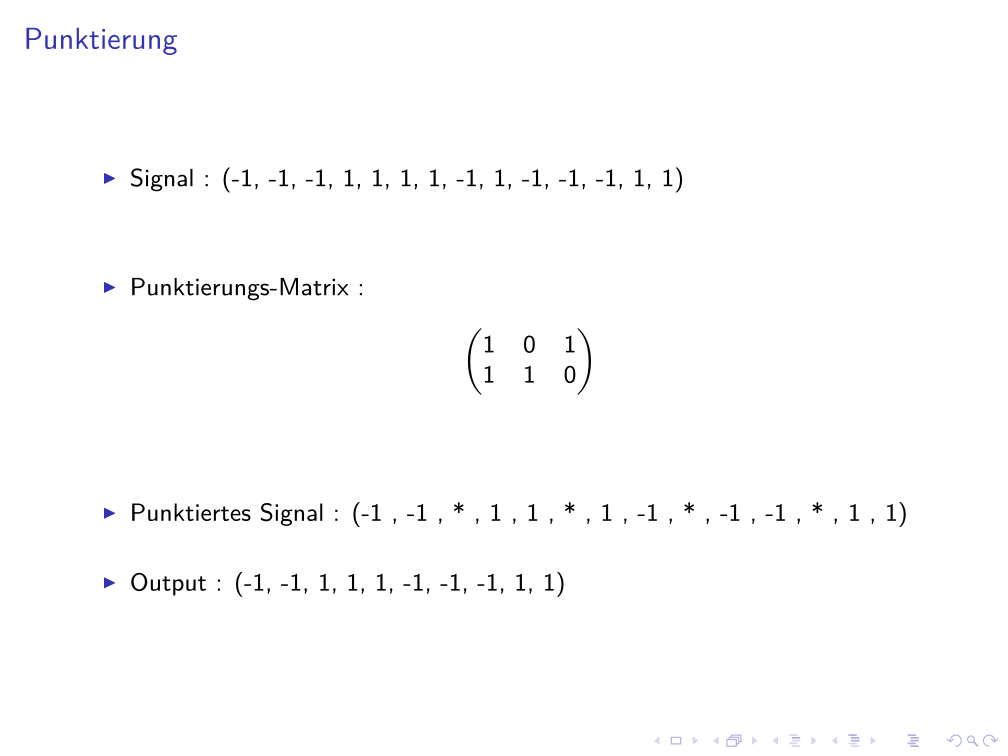
\includegraphics[width=0.7\textwidth]{abbildungen/folie_kodierung_punktierung}}
	\caption{Folie mit Punktierung}
	\label{abb:folie_punktierung}
\end{figure}
\FloatBarrier
\section{Dekodierung}
\label{kapitel:visualisierung_dekodierung}
% allg. Informationen
Bei der Dekodierung befinden sich ebenfalls, wie bei der Kodierung, allgemeine Informationen des Faltungskodierers auf den ersten Folien.
\\
% Depunktierung
Abbildung~\ref{abb:folie_depunktierung} zeigt die Folie der Depunktierung. Auf dieser wird die Depunktierung des Signals, d.h. das Einfügen des Signalwerts 0 (definiert durch die Punktierungsmatrix), dargestellt. Die eingefügten 0-Werte sind zur leichteren visuellen Erkennung farblich hervorgehoben.
\begin{figure}[th]
	\centering
	\fbox{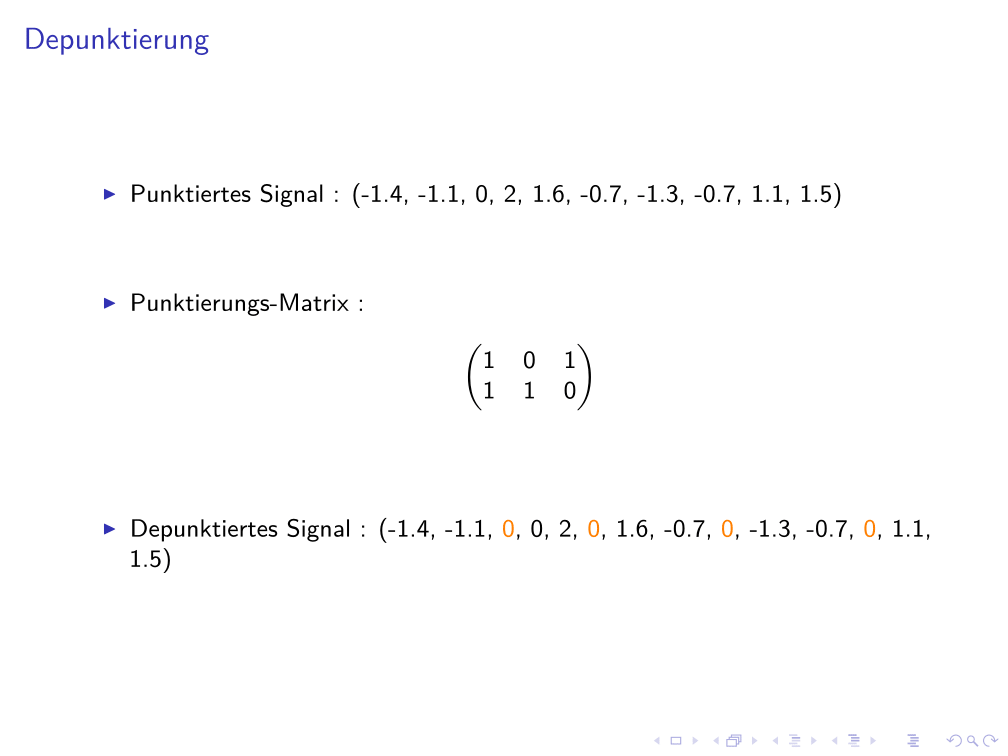
\includegraphics[width=0.7\textwidth]{abbildungen/folie_dekodierung_depunktierung}}
	\caption{Folie mit Depunktierung}
	\label{abb:folie_depunktierung}
\end{figure}
% Signal zu Kode
Als Input erhält die Dekodierung das Kodewort als kontinuierliche Signalwerte, die möglicherweise durch Anwendung der \texttt{ApplyNoise}-Funktion verfälscht worden sind. Die soft decision Dekodierung verwendet zur Dekodierung zwar direkt diese Signalwerte, da aber sowohl die hard decision Dekodierung Bitwerte zur Dekodierung verwendet, als auch die Kanten des Trellis mit Bitwerten beschriftet sind, wird der Input, um konsistent zu bleiben, auf Bitwerte abgebildet. Die Folie der Abbildung der Signalwerte auf Bitwerte (nach Gleichung~\ref{eq:signal_zu_bit_abbildung}) ist in Abbildung~\ref{abb:folie_signal_zu_bit_abbildung} zu sehen.
\begin{figure}[th]
	\centering
	\fbox{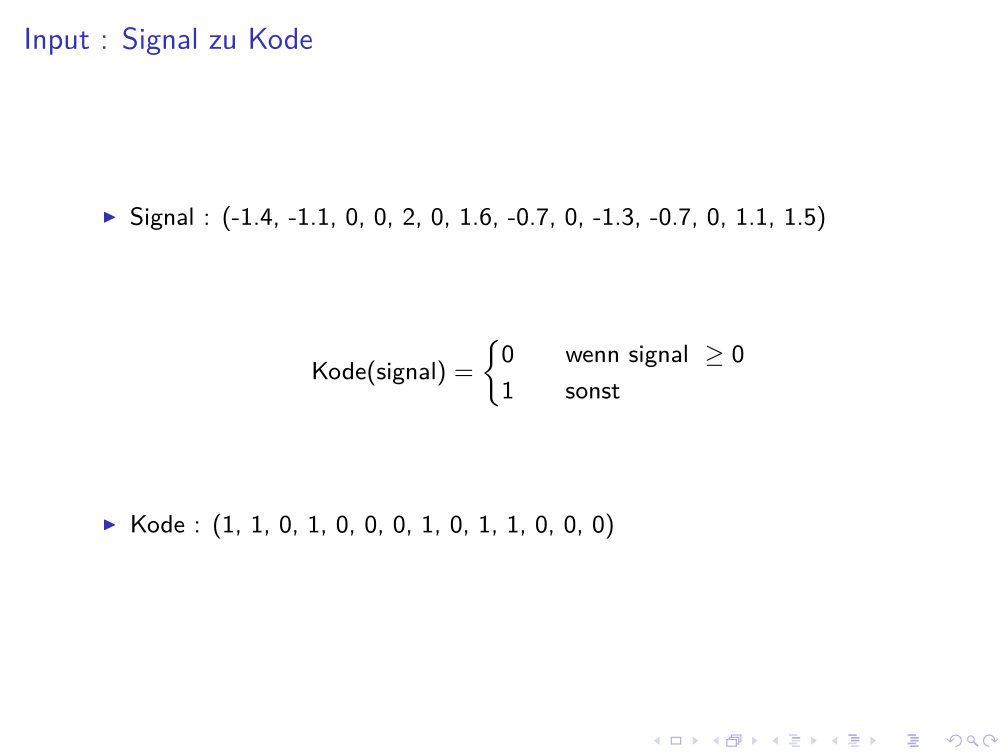
\includegraphics[width=0.7\textwidth]{abbildungen/folie_dekodierung_signal_zu_bit}}
	\caption{Folie mit der Abbildung der Signalpegel zu den Kodebits}
	\label{abb:folie_signal_zu_bit_abbildung}
\end{figure}
% Viterbi-Algorithmus
Anschließend folgt die Visualisierung des Viterbi-Algorithmus mithilfe des Trellis-Diagramms. In den farbigen Kreisen befinden sich die Metriken der Pfade, die zum jeweiligen Zustand führen. Zunächst werden, zur besseren Übersicht bei großen Diagrammen, jene Pfade entfernt, für die es eine bessere Alternative gibt. D.h. es werden jene Pfade entfernt die bei der soft decision Dekodierung eine niedrigere Metrik bzw. bei der hard decision Dekodierung eine höhere Metrik besitzen. Dieser Schritt ist zwischen den Abbildungen~\ref{abb:folie_dekodierung_1} und \ref{abb:folie_dekodierung_2} zu sehen. Danach erfolgt Schritt für Schritt die Rekonstruktion der Nachricht mittels Backtracking. Der gewählte Pfad beim Backtracking wird farblich hervorgehoben. Die übrigen Pfade werden ausgegraut. Eine Folie während des Backtrackings wird in Abbildung~\ref{abb:folie_dekodierung_3} veranschaulicht. Am Ende befindet sich unter dem Trellis-Diagramm die farblich hervorgehobene dekodierte Nachricht, wie in Abbildung~\ref{abb:folie_dekodierung_4} dargestellt. Die einzelnen Zwischenschritte vermitteln dem Benutzer wie der Algorithmus funktioniert und wie sich die dekodierte Nachricht ergibt.
\begin{figure}[th]
	\centering
	\fbox{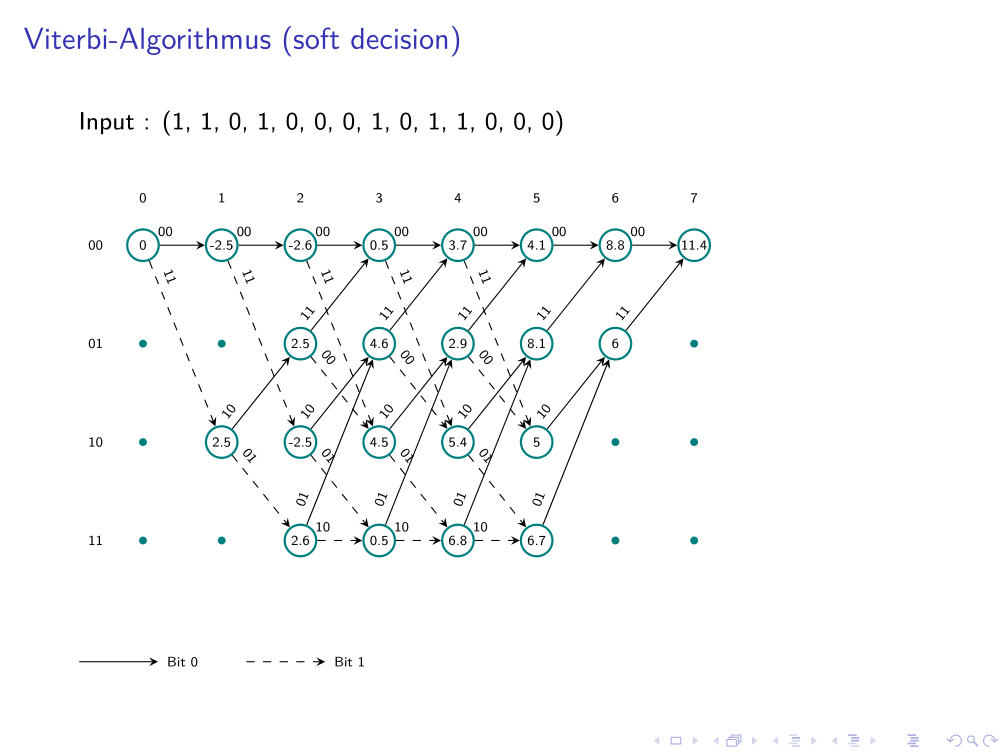
\includegraphics[width=0.7\textwidth]{abbildungen/folie_dekodierung_1}}
	\caption{Folie der soft decision Dekodierung und dem vollständigen Trellis}
	\label{abb:folie_dekodierung_1}
\end{figure}
\begin{figure}[th]
	\centering
	\fbox{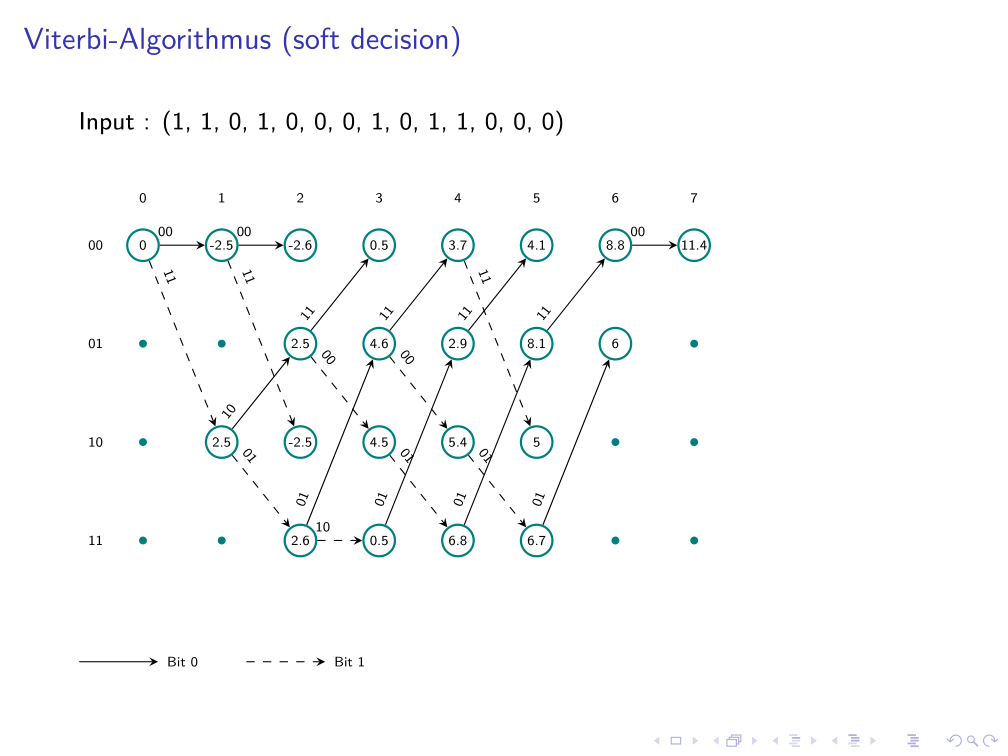
\includegraphics[width=0.7\textwidth]{abbildungen/folie_dekodierung_2}}
	\caption{Folie der soft decision Dekodierung und dem Trellis nach dem Entfernen einiger Pfade}
	\label{abb:folie_dekodierung_2}
\end{figure}
\begin{figure}[th]
	\centering
	\fbox{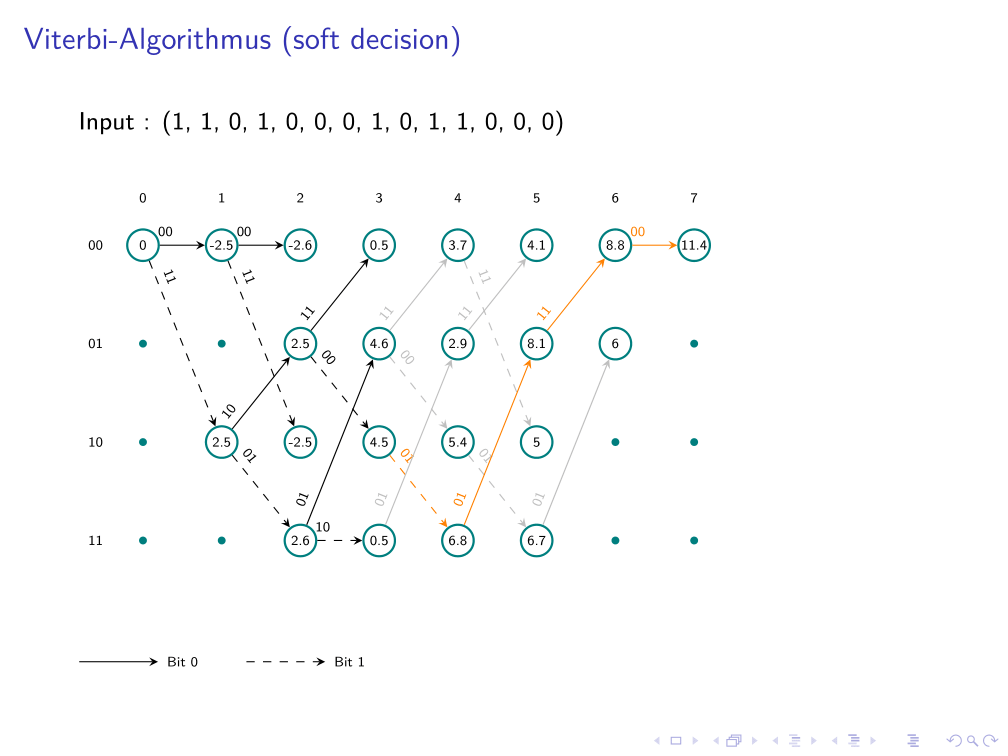
\includegraphics[width=0.7\textwidth]{abbildungen/folie_dekodierung_3}}
	\caption{Folie der soft decision Dekodierung im während dem Backtracking}
	\label{abb:folie_dekodierung_3}
\end{figure}
\begin{figure}[th]
	\centering
	\fbox{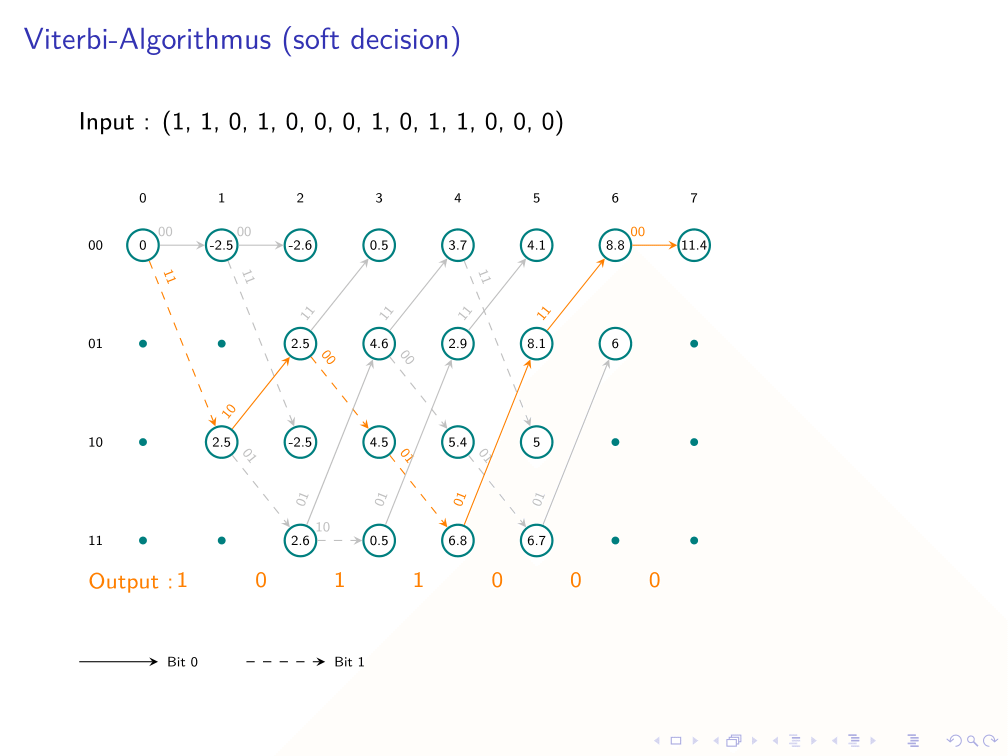
\includegraphics[width=0.7\textwidth]{abbildungen/folie_dekodierung_4}}
	\caption{Folie der soft decision Dekodierung mit der dekodierten Nachricht}
	\label{abb:folie_dekodierung_4}
\end{figure}

\section{Simulation}
\label{kapitel:visualisierung_simulation}
Auch die Simulationsfunktionen bieten durch den \texttt{visualize}-Parameter die Möglichkeit eine Visualisierung generieren zu lassen. Kapitel~\ref{kapitel:visualisierung_simulation_faltungskodierung} erläutert die Präsentation der Faltungskode-Simulation. Die Folien der Simulation verschiedener Varianten der Kanalkodierung, um diese vergleichen zu können, sind in Kapitel~\ref{kapitel:visualisierung_simulation_kanalkodierung} beschrieben.

\subsection{Faltungskodierung}
\label{kapitel:visualisierung_simulation_faltungskodierung}
Die folgenden Folien sind das Resultat der Ausführung der \texttt{ConvSimulation}-Funktion. Auf den ersten Folien sind, wie schon bei der Kodierung und Dekodierung, Informationen zum verwendeten Faltungskodierer angegeben.
\\
Anschließend folgt eine Folie mit den Eckdaten der Simulation, wie in Abbildung~\ref{abb:folie_simulation_f1} ersichtlich.
\\
Die nächste Folie, dargestellt in Abbildung~\ref{abb:folie_simulation_f2}, stellt ein Diagramm der Daten des erzeugten Dataframes dar. Die x-Achse entspricht dem Signal-Rausch-Verhältnis. Auf der y-Achse werden die gemessenen Bitfehlerraten aufgetragen. Es ist in diesem Beispiel sehr gut zu erkennen, dass die Fehleranzahl mit steigendem Signal-Rausch-Verhältnis abnimmt.
\\
Abschließend werden statistische Kennzahlen der Bitfehlerraten wie Minimum, Maximum, Median etc. auf der letzten Folie, wie in Abbildung~\ref{abb:folie_simulation_f3} zu sehen, aufgelistet. 
\begin{figure}[th]
	\centering
	\begin{subfigure}{0.48\textwidth}
		\centering
		\fbox{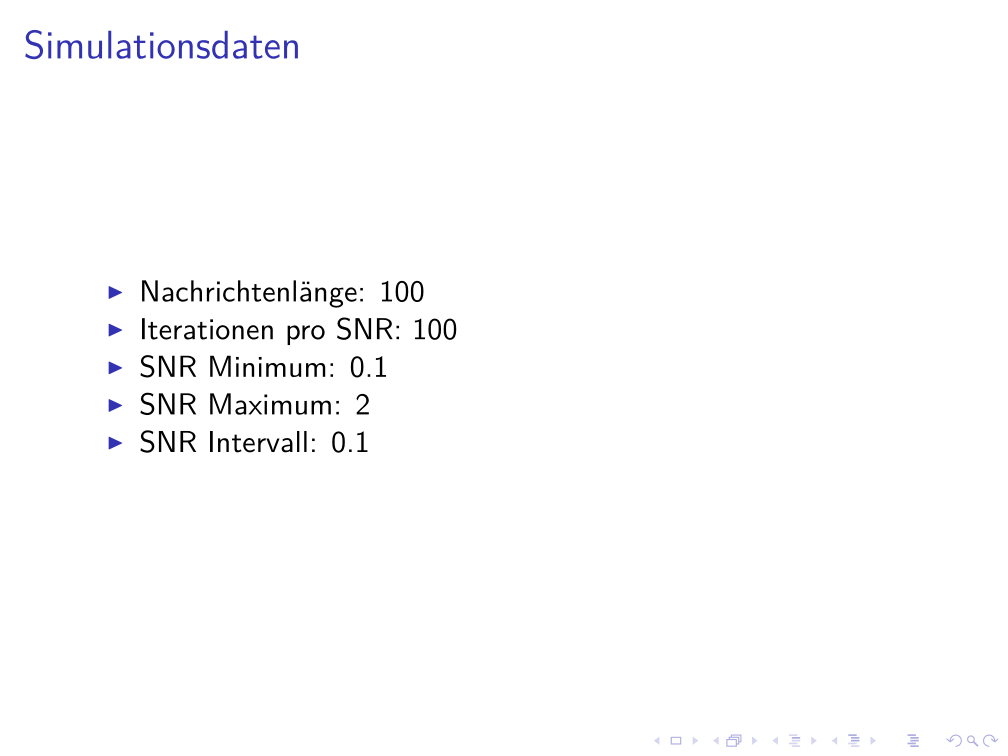
\includegraphics[width=0.99\textwidth]{abbildungen/folie_simulation_f1}}
		\caption{Folie mit Simulationseckdaten\\ \textcolor{white}{x}}
		\label{abb:folie_simulation_f1}
	\end{subfigure}
	\quad
	\begin{subfigure}{0.48\textwidth}
		\centering
		\fbox{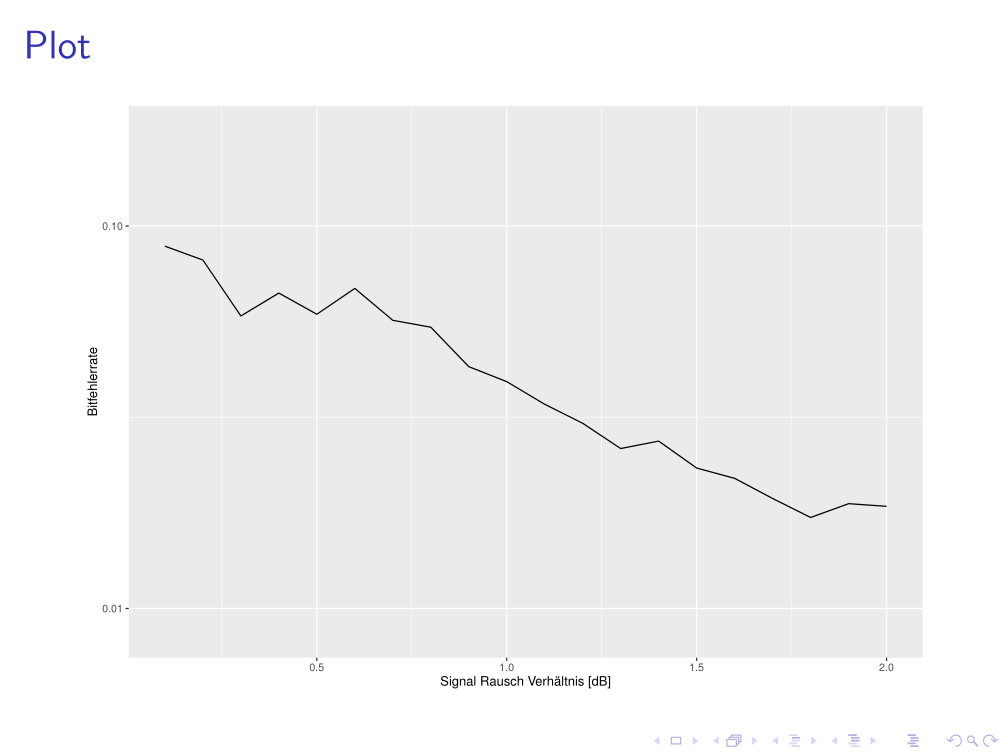
\includegraphics[width=0.99\textwidth]{abbildungen/folie_simulation_f2}}
		\caption{Folie mit Diagramm der Simulationsergebnisse}
		\label{abb:folie_simulation_f2}
	\end{subfigure}
	\par\bigskip
	\begin{subfigure}{0.48\textwidth}
		\centering
		\fbox{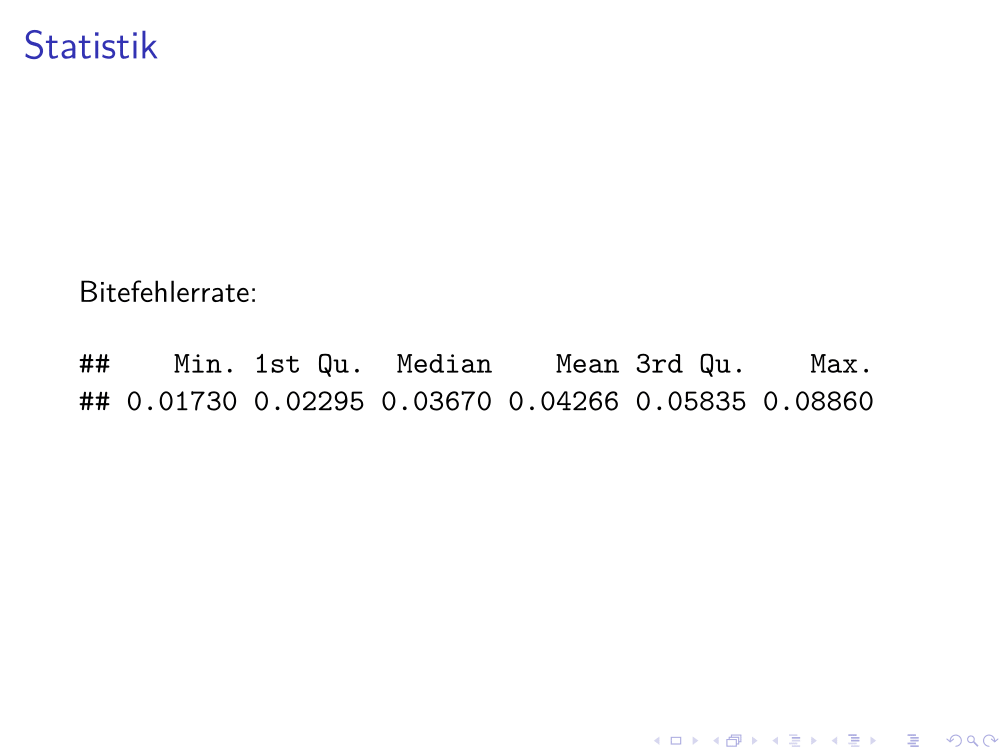
\includegraphics[width=0.99\textwidth]{abbildungen/folie_simulation_f3}}
		\caption{Folie mit Statistik der Bitfehlerraten}
		\label{abb:folie_simulation_f3}
	\end{subfigure}
	\caption{Folien der Faltungskodierungs-Simulation}
	\label{abb:folie_simulation_f}
\end{figure}

\subsection{Kanalkodierung}
\label{kapitel:visualisierung_simulation_kanalkodierung}
\begin{figure}[th]
	\centering
	\begin{subfigure}{0.48\textwidth}
		\centering
		\fbox{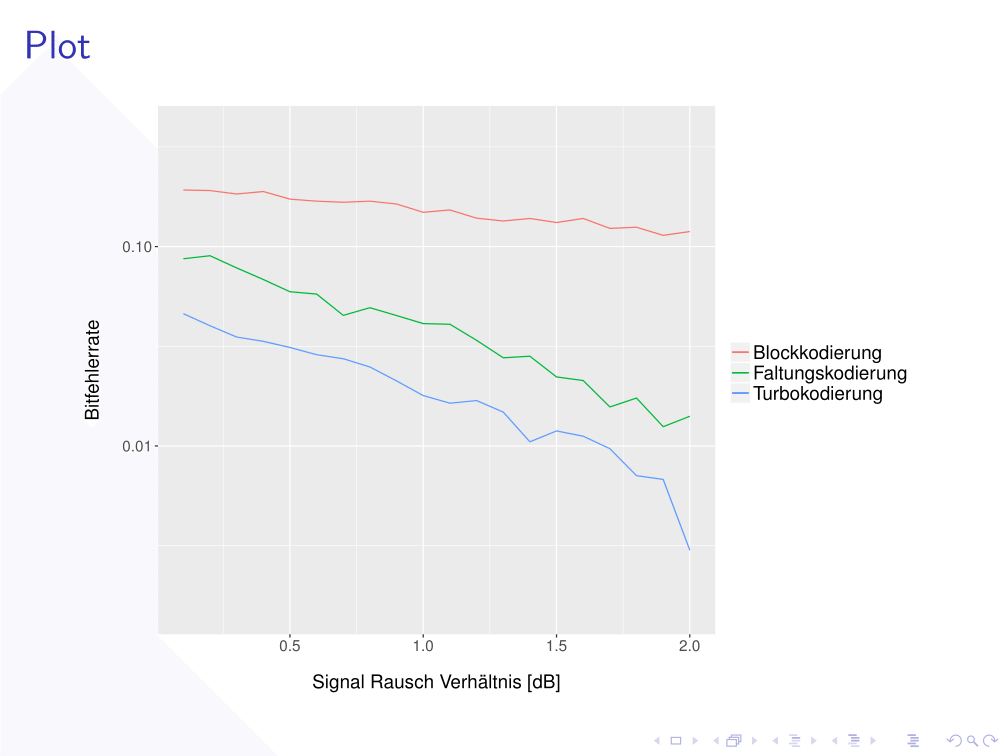
\includegraphics[width=0.99\textwidth]{abbildungen/folie_simulation_k1}}
		\caption{Folie mit Diagramm der Ergebnisse}
		\label{abb:folie_simulation_k1}
	\end{subfigure}
	\quad
	\begin{subfigure}{0.48\textwidth}
		\centering
		\fbox{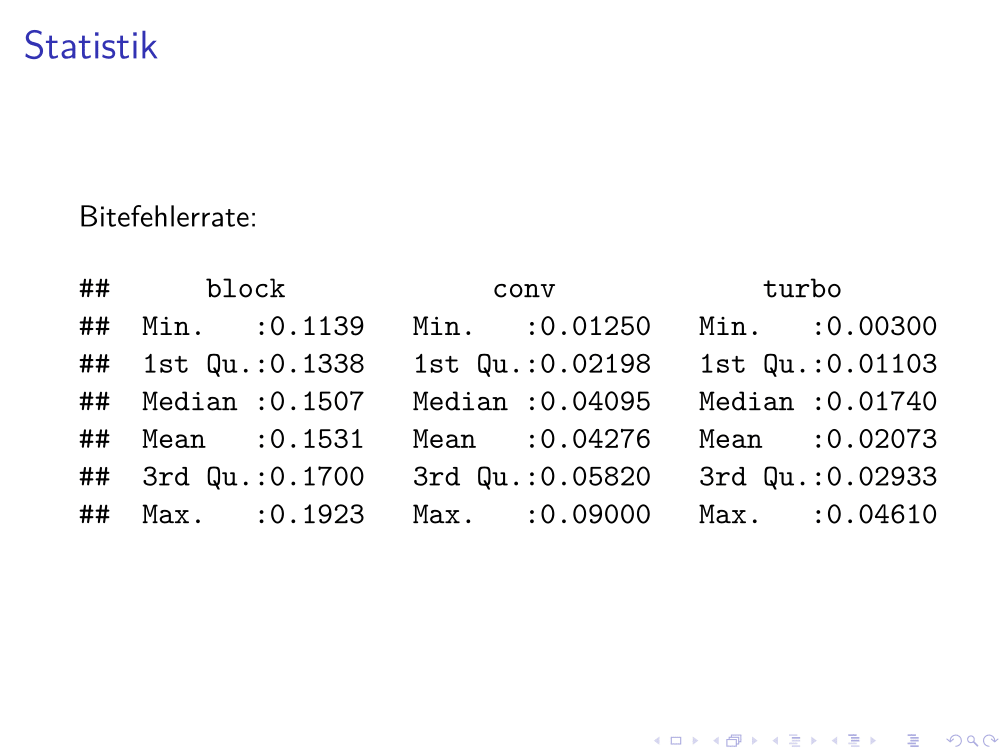
\includegraphics[width=0.99\textwidth]{abbildungen/folie_simulation_k2}}
		\caption{Folie mit Simulationsstatistik}
		\label{abb:folie_simulation_k2}
	\end{subfigure}
	\caption{Folien der Kanalkodierungs-Simulation}
	\label{abb:folie_simulation_k}
\end{figure}
Für einen Vergleich der im R-Paket implementierten Verfahren der Kanalkodierung kann die \texttt{ChannelcodingSimulation}-Funktion ausgeführt werden, deren Simulationsergebnisse ebenfalls dargestellt werden können. Zu Beginn der Kanalkodierungs-Visualisierungen werden auf einer Folie die Simulationseckdaten aufgelistet, wie es schon bei der Visualisierung der Faltungskodierungs-Simulation der Fall war.
\\
Abbildung~\ref{abb:folie_simulation_k1} zeigt die Folie mit dem Diagramm, in dem die Ergebnisse der drei Simulationen dargestellt werden und miteinander verglichen werden können. Die Art der Kodierung einer Kurve kann anhand der Farbe zugeordnet werden.
%\begin{figure}[th]
%	\centering
%	\fbox{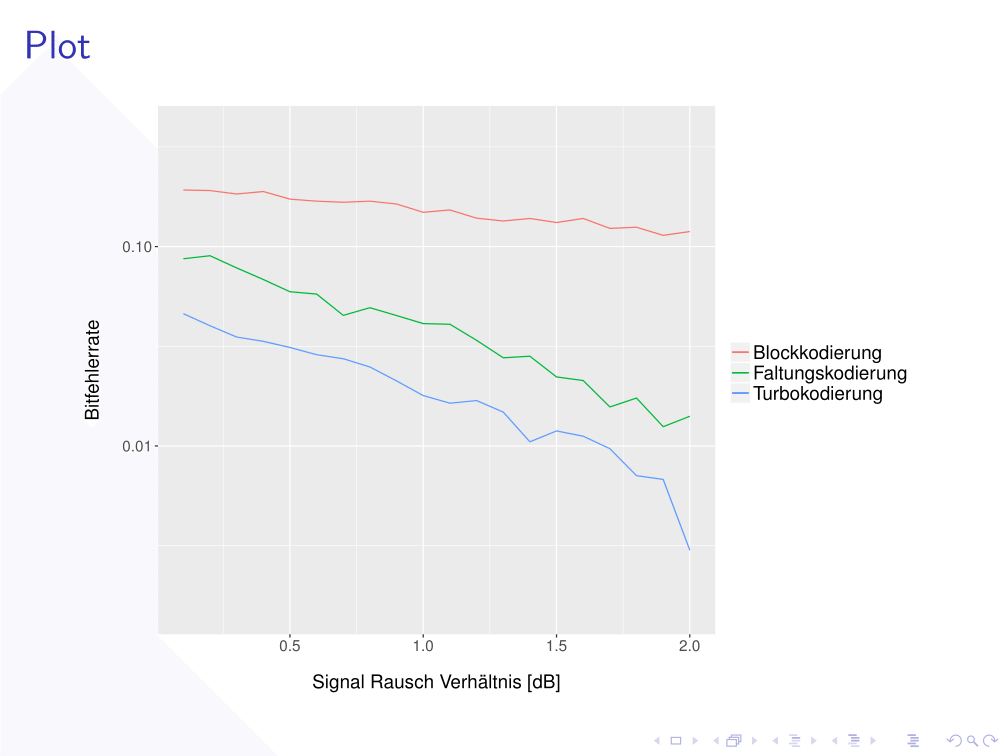
\includegraphics[width=0.7\textwidth]{abbildungen/folie_simulation_k1}}
%	\caption{Folie mit Diagramm der Ergebnisse der Kanalkodierungs-Simulationen}
%	\label{abb:folie_simulation_k1}
%\end{figure}
Wie auch schon in Kapitel~\ref{kapitel:visualisierung_simulation_faltungskodierung} befindet sich auf der letzten Folie eine Statistik der Bitfehlerraten. Dabei werden die Werte der verschiedenen Kanalkodierungs-Varianten gegenübergestellt. Abbildung~\ref{abb:folie_simulation_k2} zeigt ein Beispiel zur Statistik-Folie.
%\begin{figure}[th]
%	\centering
%	\fbox{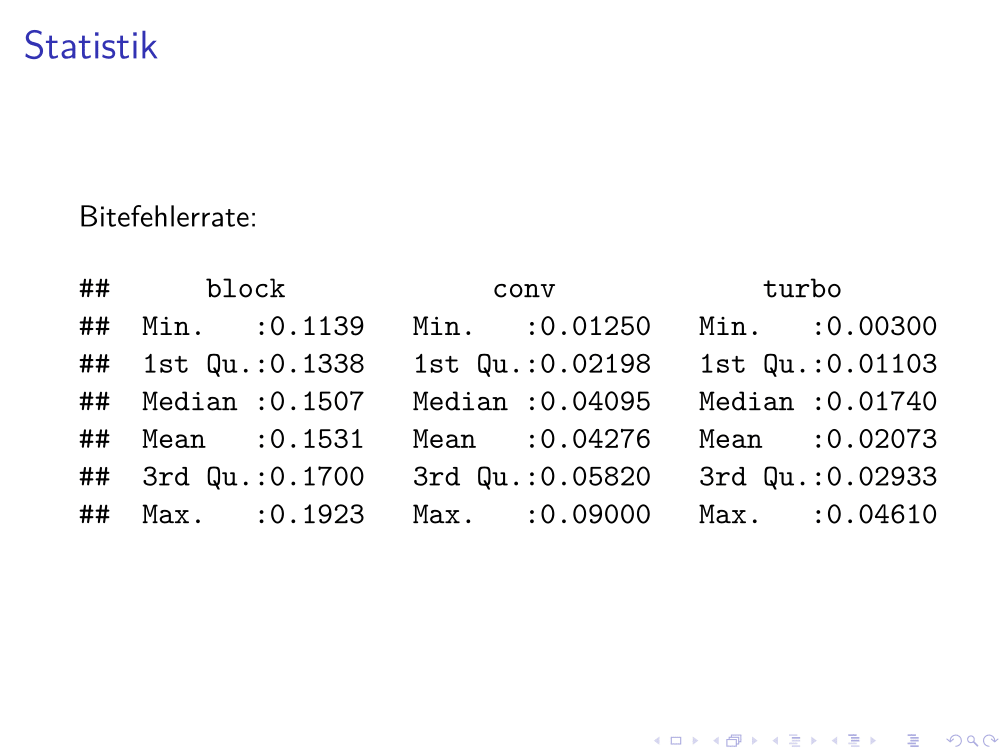
\includegraphics[width=0.7\textwidth]{abbildungen/folie_simulation_k2}}
%	\caption{Folie mit Simulationsstatistik}
%	\label{abb:folie_simulation_k2}
%\end{figure}

\chapter{Beispiele}
\label{kapitel:beispiele}

\chapter{Fazit, Ausblick, Erweiterungen}
\label{kapitel:fazit}

\cleardoublepage%

\listofabbreviations
\clearpage

\listoffigures
\clearpage

\printlist[Funktionen]{lot}{}{\renewcommand\addvspace[1]{}\chapter*{Funktionsverzeichnis}}
\clearpage

%\listoftables
%\clearpage

\lstlistoflistings
\clearpage

\printbibliography
\end{document}
